\documentclass[a4paper]{article}

\usepackage{geometry}
\geometry{left=2.5cm, right=2.5cm, top=2.5cm, bottom=2.5cm}

\usepackage{ctex}
\zihao{-4}

\usepackage{amsmath}
\usepackage{siunitx}
\usepackage[version=4]{mhchem}

\usepackage{enumitem}
\usepackage{multirow}
\usepackage{adjustbox}
\usepackage[hidelinks]{hyperref}

\usepackage{tabularx}
\usepackage{array}
\newcolumntype{Y}{>{\centering\arraybackslash}X}

\usepackage{float}
\usepackage{caption}
\usepackage{graphicx}

\usepackage{tikz}
\usepackage[siunitx]{circuitikz}


\begin{document}

\noindent\textbf{班级：24级整合科学班} \hspace{1cm} \textbf{学号：2400017802} \hspace{1cm} \textbf{姓名：冯翊展} \hspace{1cm} \textbf{评分：}\\
\textbf{同组学生：无} \\
\textbf{实验名称：光电二极管与碘钟反应}   \hfill \textbf{实验日期：2025年5月30日} 

\vspace{0.5mm}
\hrule
\vspace{3mm}

\begin{enumerate}[label=\chinese*.,left=0pt]
    \item 实验目的
        \begin{enumerate}[label=\arabic*.,left=0pt]
            \item 了解光电二极管（PD）的特性，组装光强测量电路。
            \item 学习焊接，组装LED-PD联合电路，并与比色皿、NI DAQ 搭配构成简易分光光度计。
            \item 使用简易分光光度计监测碘钟反应的反应速率与周期数。
        \end{enumerate}

    \item 基本原理
        \begin{enumerate}[label=\arabic*.,left=0pt]
            \item 光电二极管
            \\[1mm]
            光电二极管（Photo-Diode，简称PD）是一种将光信号转换为电信号的半导体器件。光电二极管的管芯是一个具有光敏性质的PN结，工作时需加上反向电压。无光照时，有很小的饱和反向漏电流，称为暗电流，此时光敏二极管截止；受到光照时由于光电效应，饱和反向漏电流大大增加，形成光电流，且输出电流与入射光强度大致成正比。光电二极管的工作曲线如图~\ref{PDWC} 所示。

            \begin{minipage}[t]{0.5\textwidth}
                \centering
                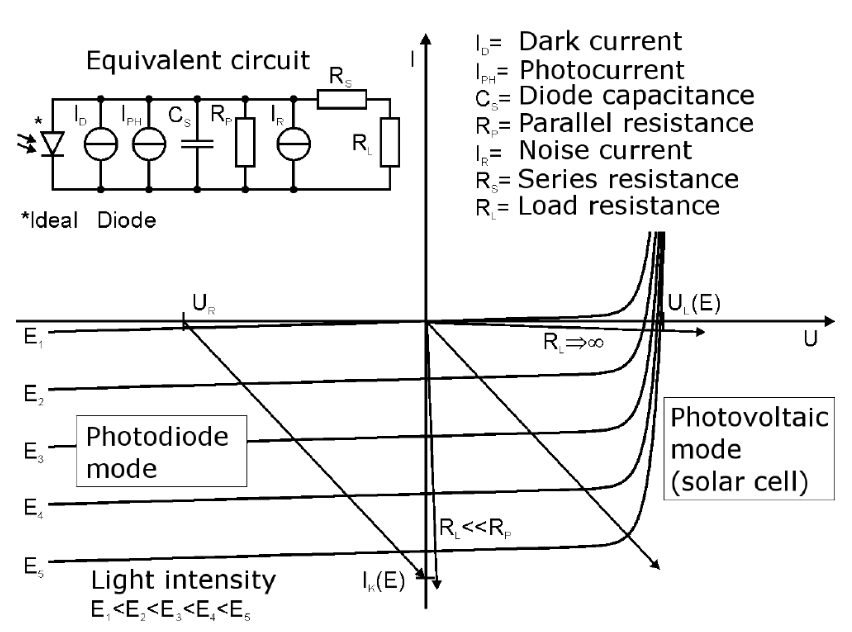
\includegraphics[width=\textwidth]{PD Work Curve.png}
                \captionof{figure}{光电二极管工作曲线}
                \label{PDWC}
            \end{minipage}
            \hfill
            \begin{minipage}[t]{0.4\textwidth}
                \centering
                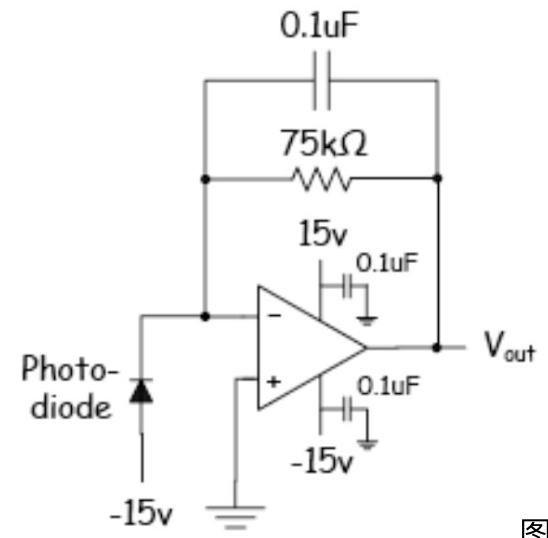
\includegraphics[width=\textwidth]{PD Circuit.png}
                \captionof{figure}{光电二极管电流-电压转换电路}
                \label{PD Circuit}
            \end{minipage}
            \\[5mm]
            一般光电二极管的输出光电流在$\qty{}{\nA} \sim \qty{}{\uA}$级别，因此需要使用运算放大器将电流信号放大并转换为电压信号输出，相应电路如图~\ref{PD Circuit} 所示。

            \item 碘钟反应
            \\[1mm]
            碘钟反应是一类典型的震荡反应，即反应过程中某组分的浓度不呈现单调变化，而是周期性变化的现象。实验所使用的反应体系包含三种反应物：过氧化氢、丙二酸与碘酸钾，另外包含催化剂硫酸锰和硫酸，以及指示剂淀粉。反应过程可看作是多个反应的循环：
            \begin{align*}
                \ce{2IO^-_3 + 5 H_2O_2 + 2 H^+ &-> I_2 + 5 O_2 + 6 H_2O} \\
                \ce{I_2 + CH_2(COOH)_2& -> CHI(COOH)_2 + H^+ + I^-} \\
                \ce{2CHI(COOH)_2 + 7H_2O_2 &-> 6CO_2 + I_2 + 10H2O}\\
                \ce{2I^- + H2O2 + 2H+&-> I_2 + 2H2O}
            \end{align*}
            反应过程中，碘单质的浓度出现周期性的震荡，由于其可与淀粉形成蓝色复合物，溶液的颜色也出现周期性的改变。
            
        \end{enumerate}
    
    \item 仪器与试剂
        \begin{enumerate}[label=\arabic*.,left=0pt]
            \item 仪器：LED-PD联合电路（运算放大器、反光二极管、光电二极管、定值电阻、电容、导线），学生电源，信号发生器、NI DAQ，万用表，电路板，电烙铁，焊锡，比色皿，比色皿支架，滴管。
            \item 试剂：溶液A（$\qty{3.6}{\mol \per \L}$ 过氧化氢溶液），溶液B（$\qty{0.15}{\mol \per \L}$ 丙二酸、$\qty{0.02}{\mol \per \L}$ 硫酸锰和 $0.03\%$淀粉混合溶液），溶液C（$\qty{0.2}{\mol \per \L}$ 碘酸钾和 $\qty{0.08}{\mol \per \L}$ 硫酸混合溶液）。
        \end{enumerate}

    \item 实验步骤
        \begin{enumerate}[label=\arabic*.,left=0pt]
            \item 光电二极管电路
            \begin{enumerate}[label=(\alph*),left=0pt]
                \item 在面包板上组装如图~\ref{PD Circuit} 所示的电路；
                \item 使用万用表测量有环境光照、PD被遮挡（无光照）和使用LED对PD光照时，运放输出端的电压大小；
                \item 使用信号发生器提供 $\qty{1}{} \sim \qty{3}{\V}$ 的信号给LED电路，观察PD电路运放的输出变化；在$\qty{1}{} \sim \qty{1000}{\Hz}$间改变信号频率，观察PD电路运放的输出变化；尝试摘除PD电路中负反馈电容，再重复上面的频率变化，观察PD电路运放的输出变化。
            \end{enumerate}

            \item 碘钟实验
            \begin{enumerate}[label=(\alph*),left=0pt]
                \item 使用锡焊技术将LED-PD电路焊接到电路板上，并将比色皿支架粘接到电路板上，放入比色皿，将电路与NI DAQ连接；
                \item 使用滴管向比色皿中加入溶液B和C各 $\qty{1}{\mL}$，混合后再加入A$\qty{1}{\mL}$溶液，观察现象并使用LabVIEW读取电路输出电压信号；
                \item 待溶液颜色变为紫黑色且产生大量气泡后，停止记录数据，将反应完的溶液倒入废液缸。
            \end{enumerate}
        \end{enumerate}

    \item 实验结果与分析
    \begin{enumerate}[label=\arabic*.,left=0pt]
        \item 光电二极管电路
        \\[1mm]
        实际搭建电路如图~\ref{actual circuit}，其中运放正输入端接地，因此由运放的特性可知，其负输入端的电势为$\qty{0}{\V}$，故光电二极管两端有$\qty{-15}{\V}$的反向电压。在光照下，光电二极管反向导通产生光电流，电流流经定值电阻，转换为$V_\text{out}$被NI DAQ测得。实际电路测得，环境光照下$V_\text{out} = \qty{2.072}{\V}$，PD被遮挡时$V_\text{out} = \qty{0.059}{\V}$，使用LED直接照射时$V_\text{out} = \qty{14.15}{\V}$。
        \\[3mm]
        \begin{minipage}{\linewidth}
            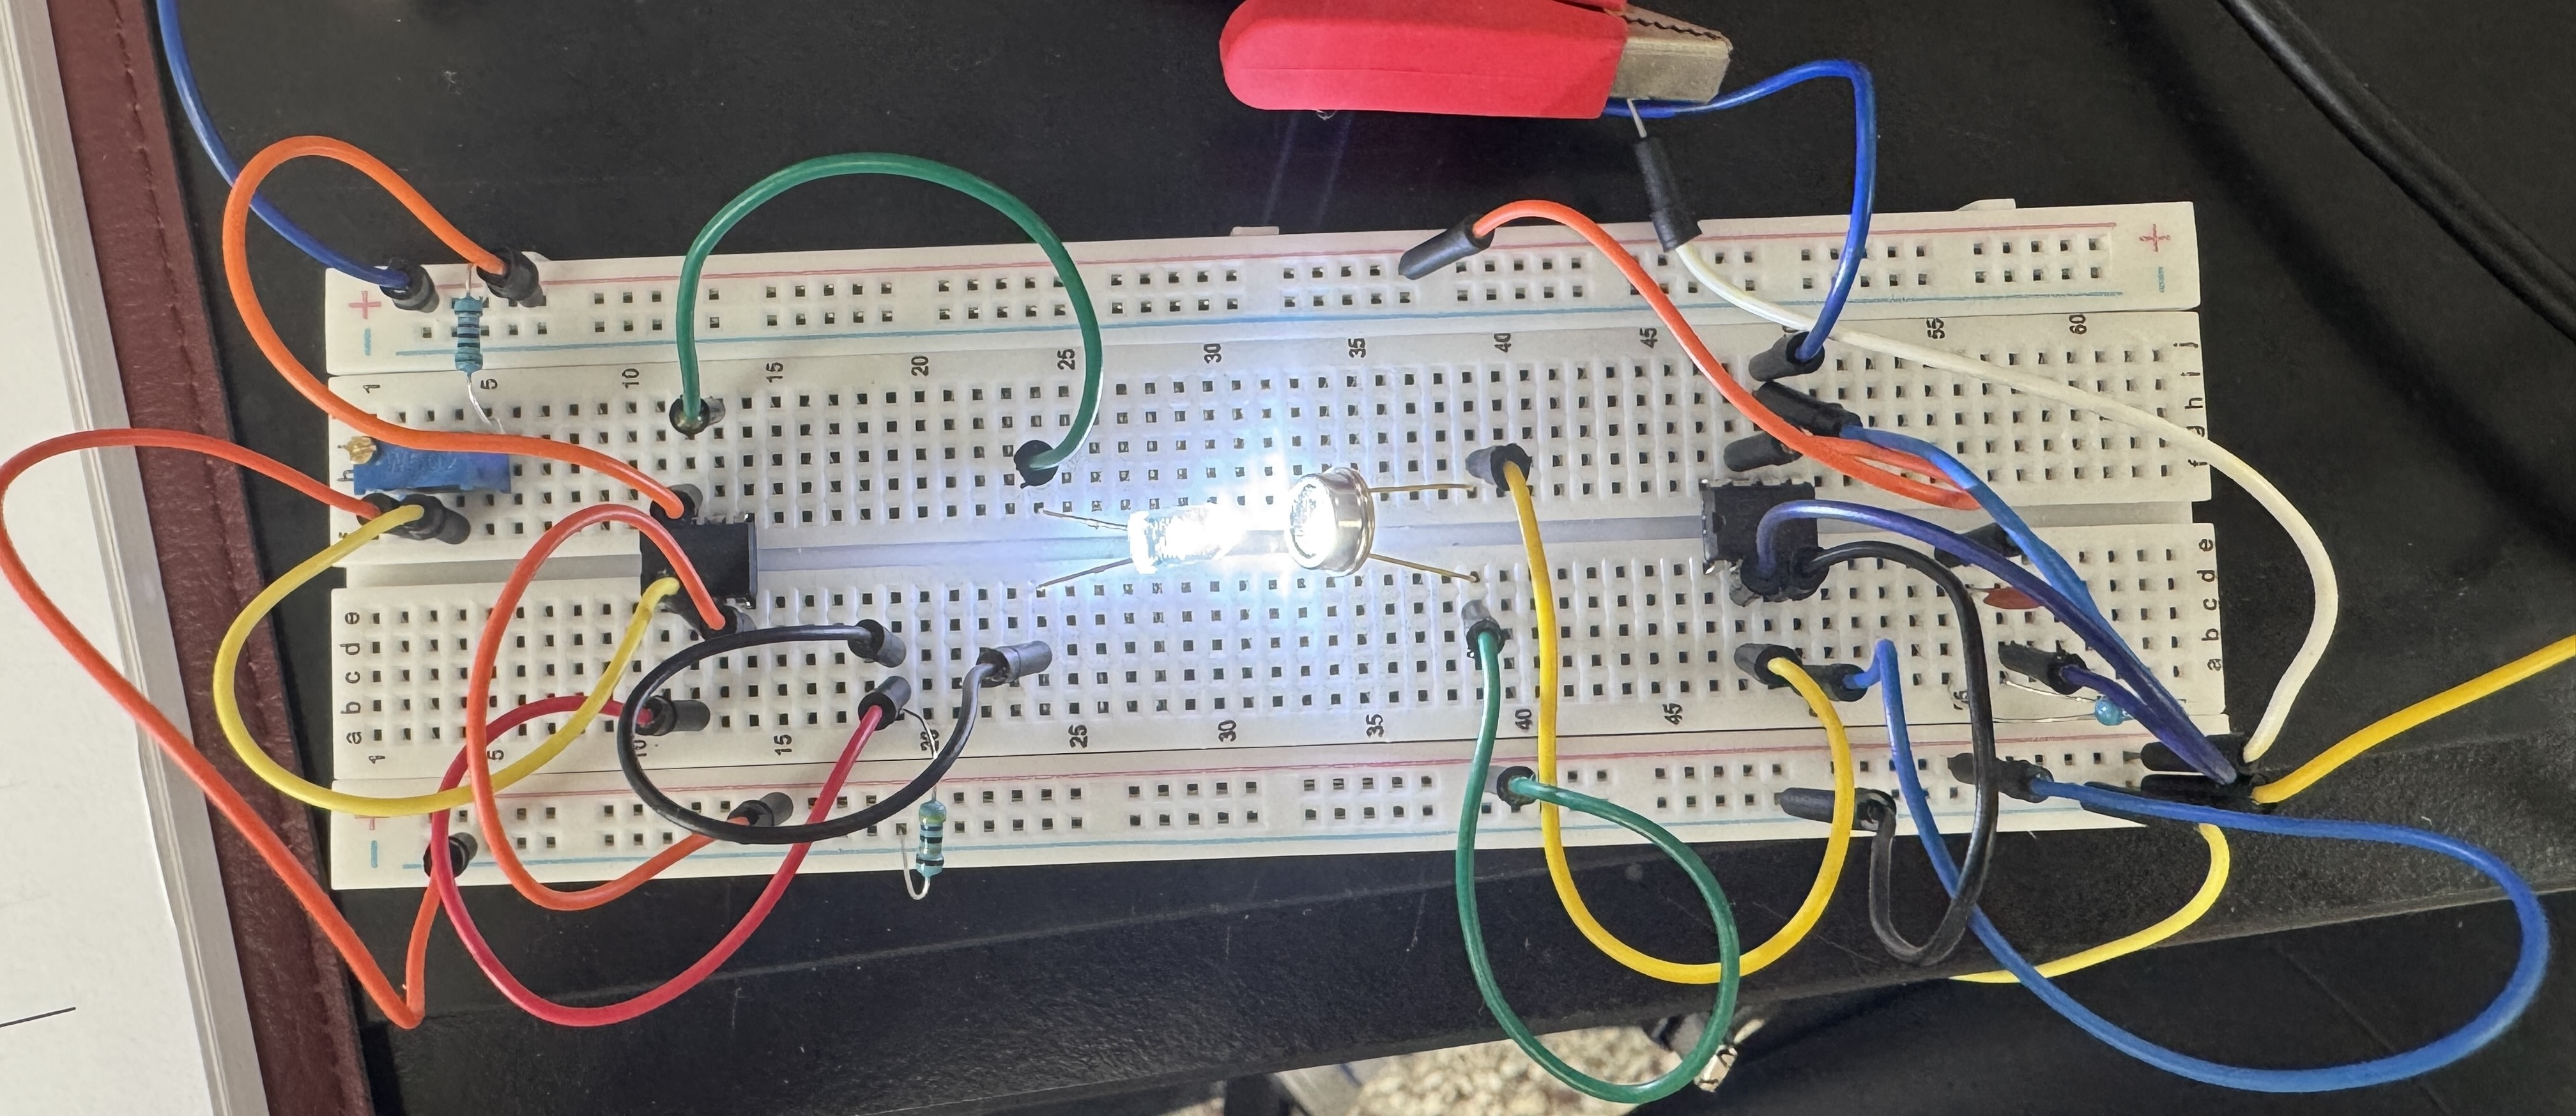
\includegraphics[width=0.9\linewidth]{Actual Circuit.jpg}
            \centering
            \captionof{figure}{实际电路}
            \label{actual circuit}
        \end{minipage}
        \\[4mm]
        将LED电路的直流电压输入换为信号发生器产生的正弦波电压。首先固定输入电压频率为 $\qty{1}{\Hz}$，调整振幅为 $\qty{\pm1}{} \sim \qty{\pm3}{\V}$，记录PD电路 $V_\text{out}$曲线如图~\ref{diffV}。观察到输出电压曲线为类半正弦波，频率基本相同但是振幅与输入电压振幅正相关。
        \\[3mm]
        \begin{minipage}{\linewidth}
            \centering
            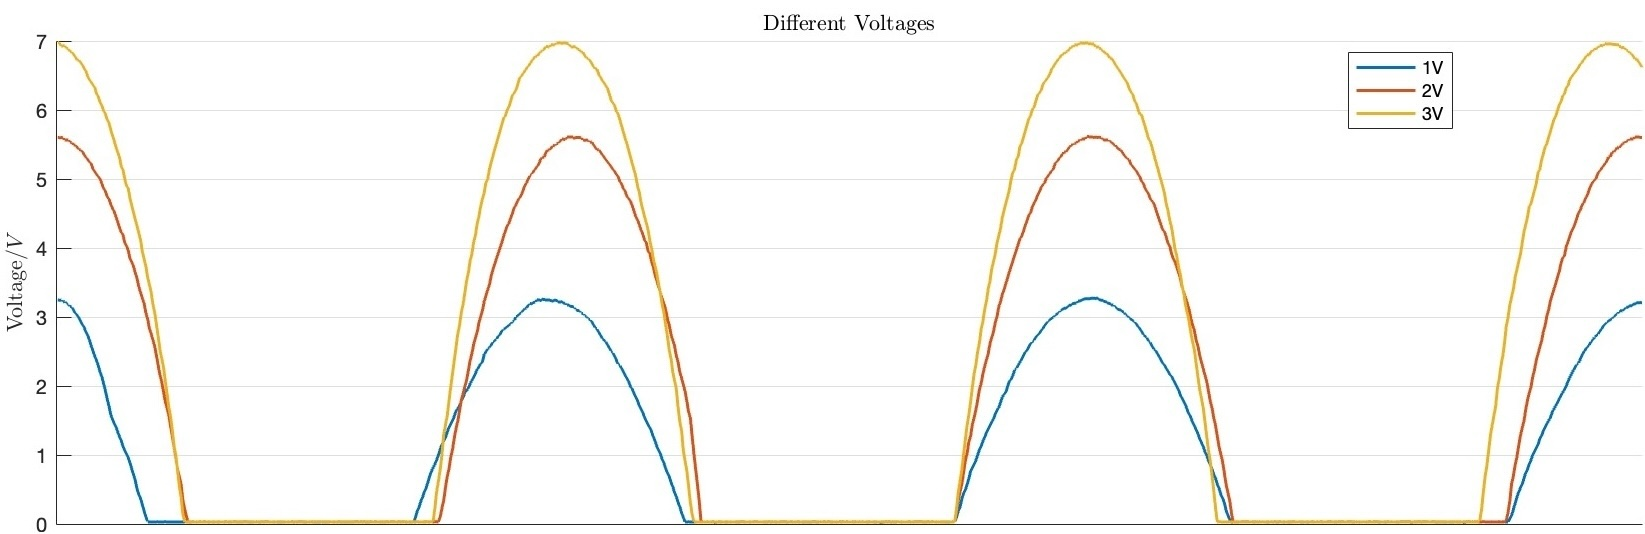
\includegraphics[width=0.85\linewidth]{Different Voltages.jpg}
            \captionof{figure}{不同输入电压比较}
            \label{diffV}
        \end{minipage}
        \\[3mm]
        再固定输入电压振幅，调整频率为 $\qty{5}{} \sim \qty{1000}{Hz}$，记录PD电路 $V_\text{out}$曲线如图~\ref{diffFreq}。观察到输出电压频率与输入频率正相关，频率超过$\qty{50}{\Hz}$后，已经接近运放最快响应速度和 NI DAQ最快信号捕获频率，因此捕获的波形逐渐不完整。
        \\[6mm]
        \begin{minipage}{\linewidth}
            \centering
            \begin{minipage}[t]{0.32\textwidth}
                \centering
                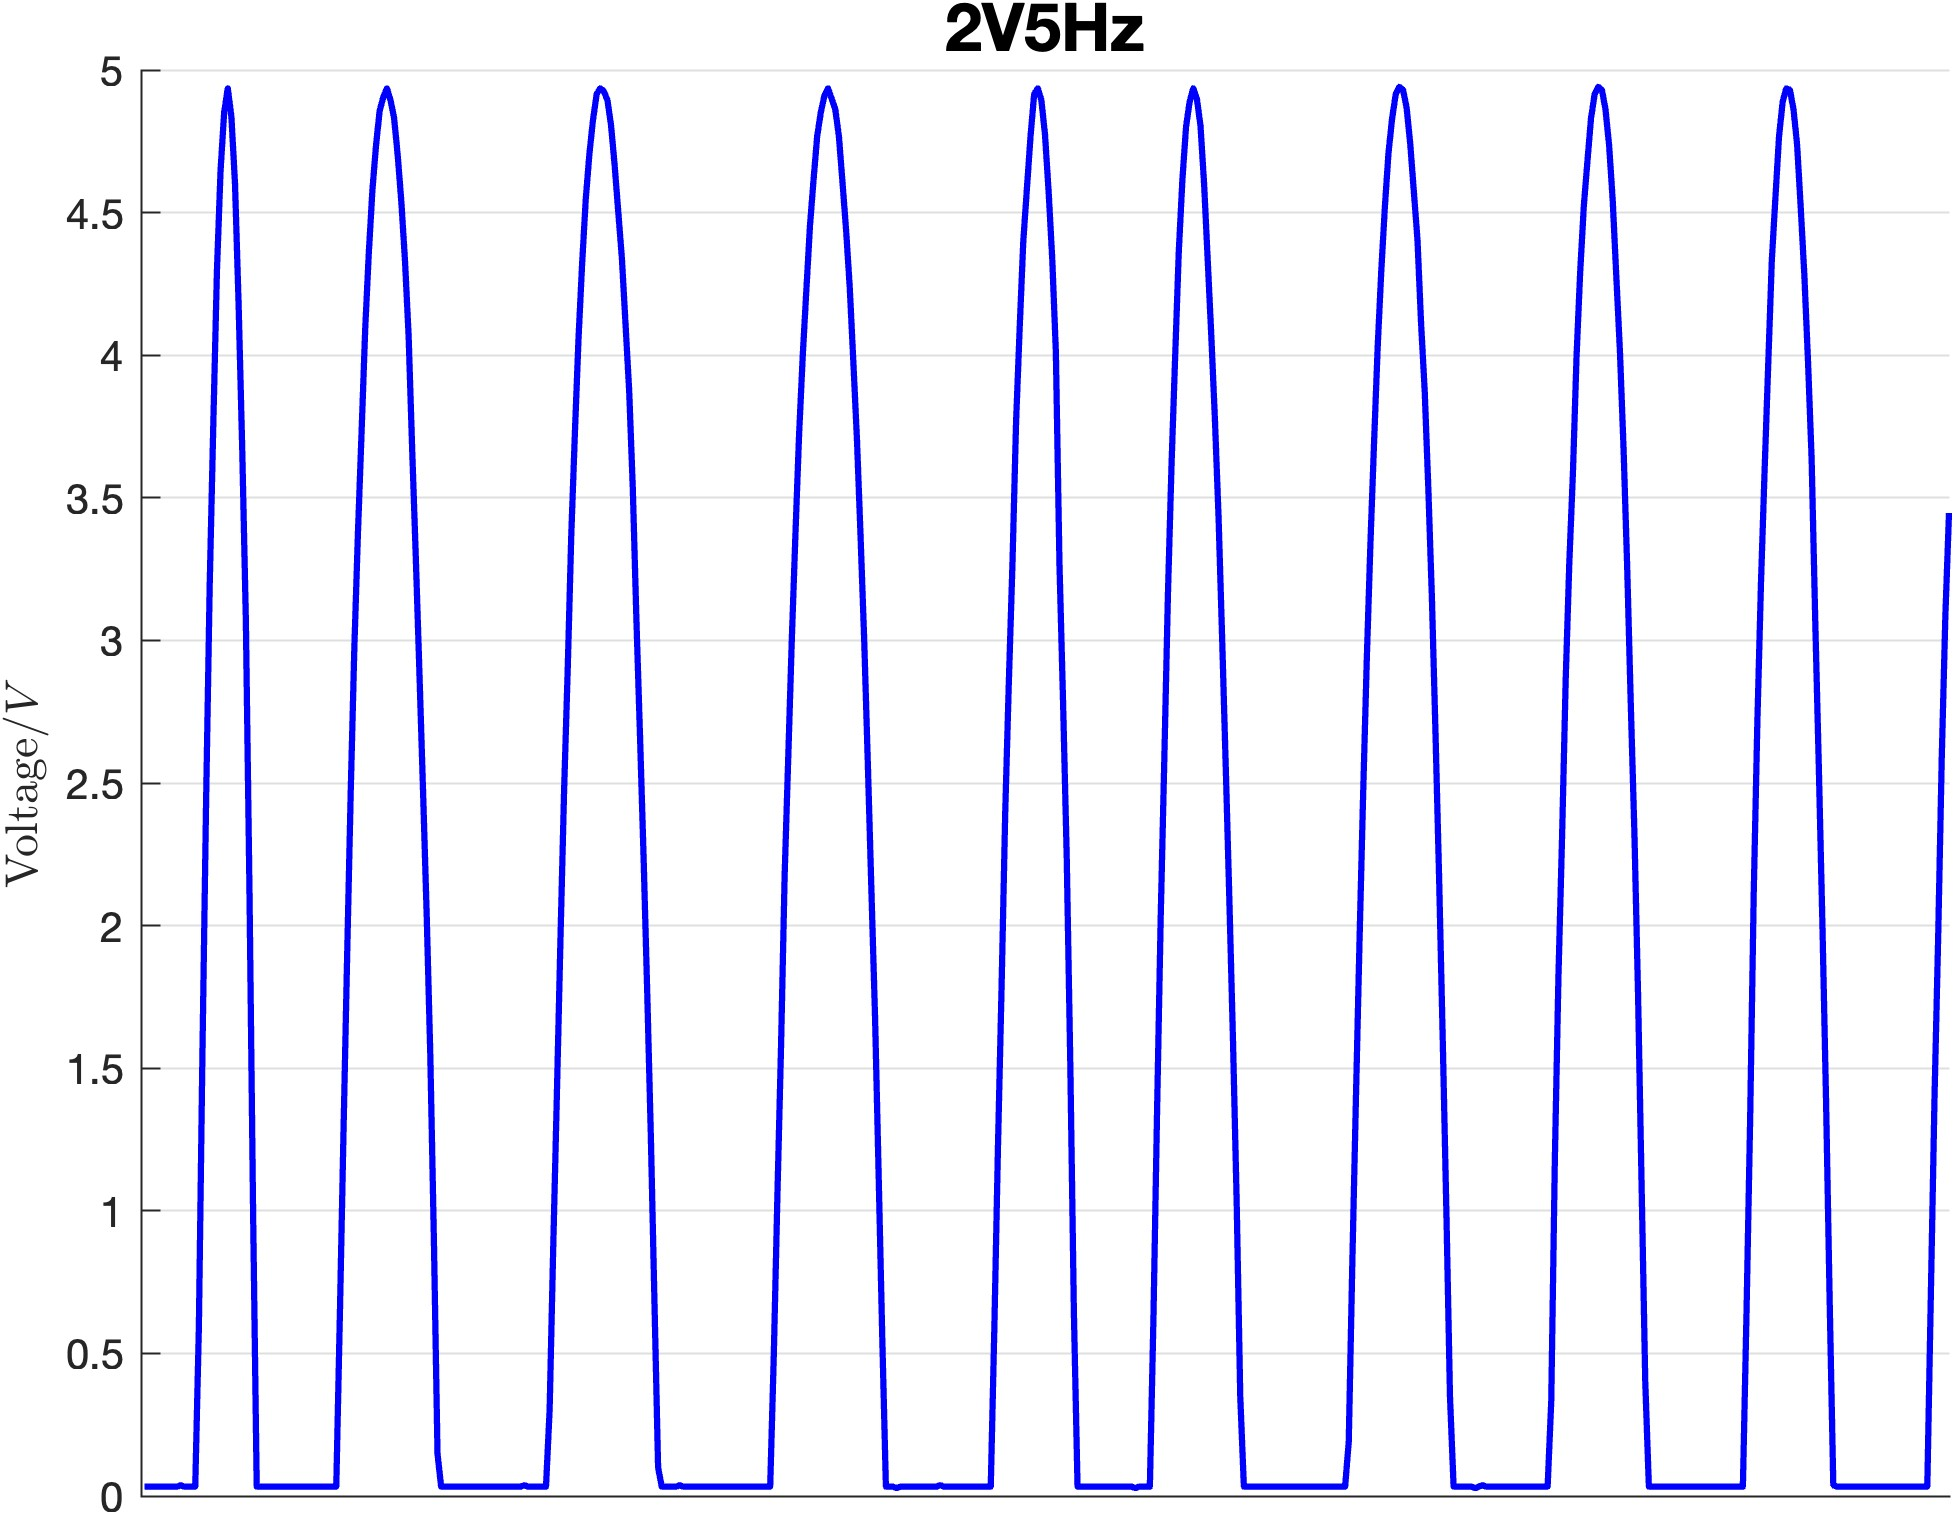
\includegraphics[width=\textwidth]{2V5Hz.jpg}
            \end{minipage}
            %\hfill
            \begin{minipage}[t]{0.32\textwidth}
                \centering
                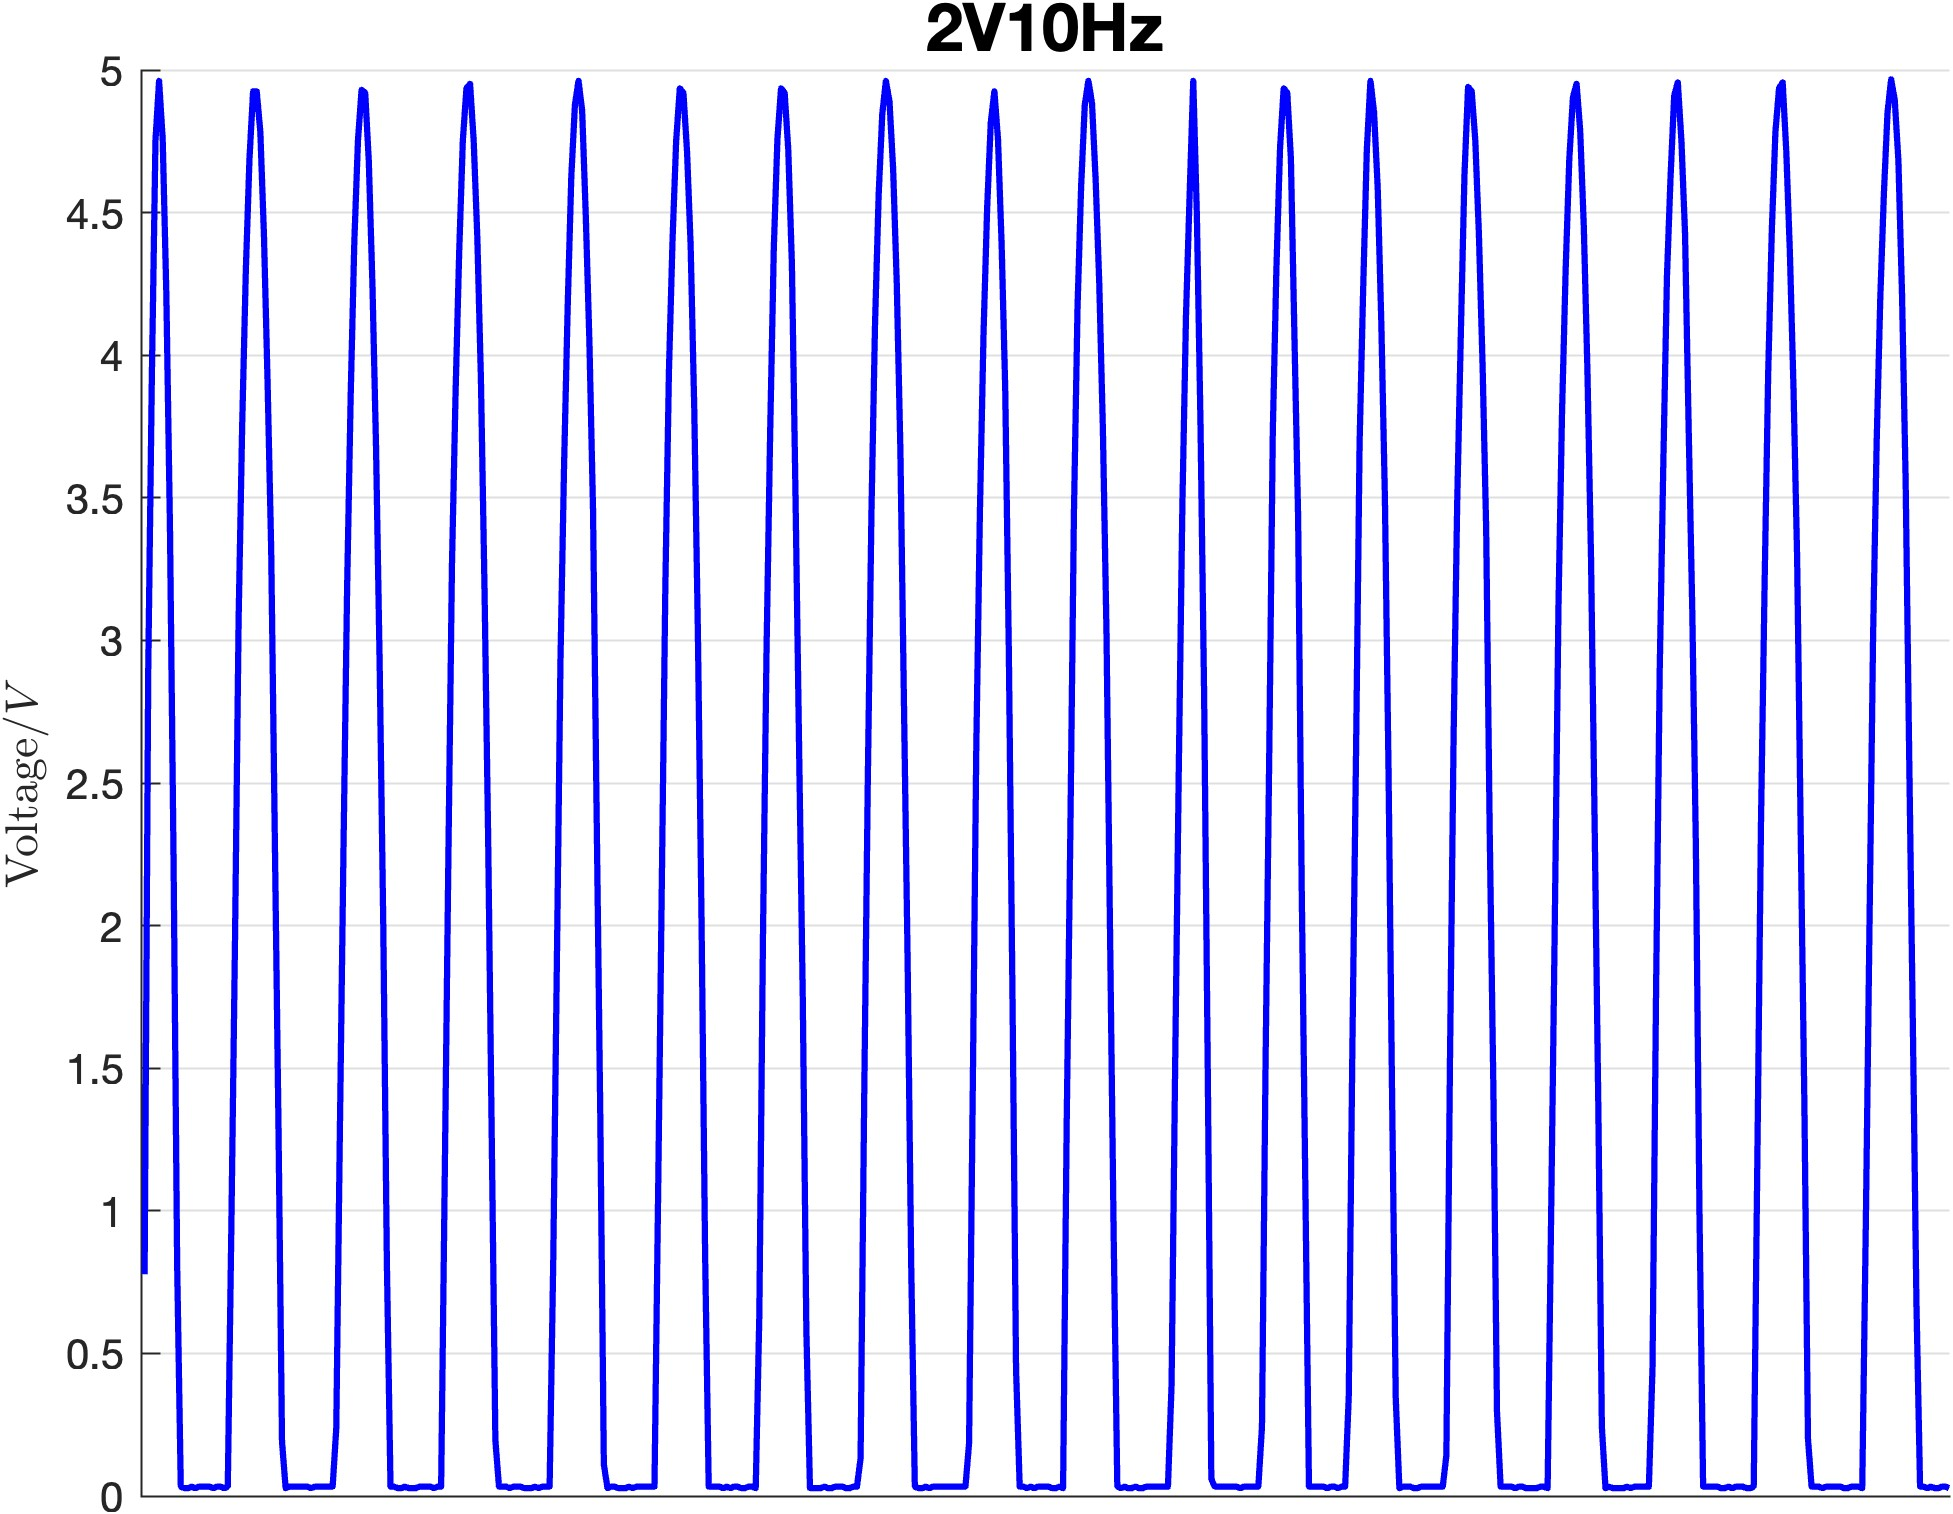
\includegraphics[width=\textwidth]{2V10Hz.jpg}
            \end{minipage}
            %\hfill
            \begin{minipage}[t]{0.32\textwidth}
                \centering
                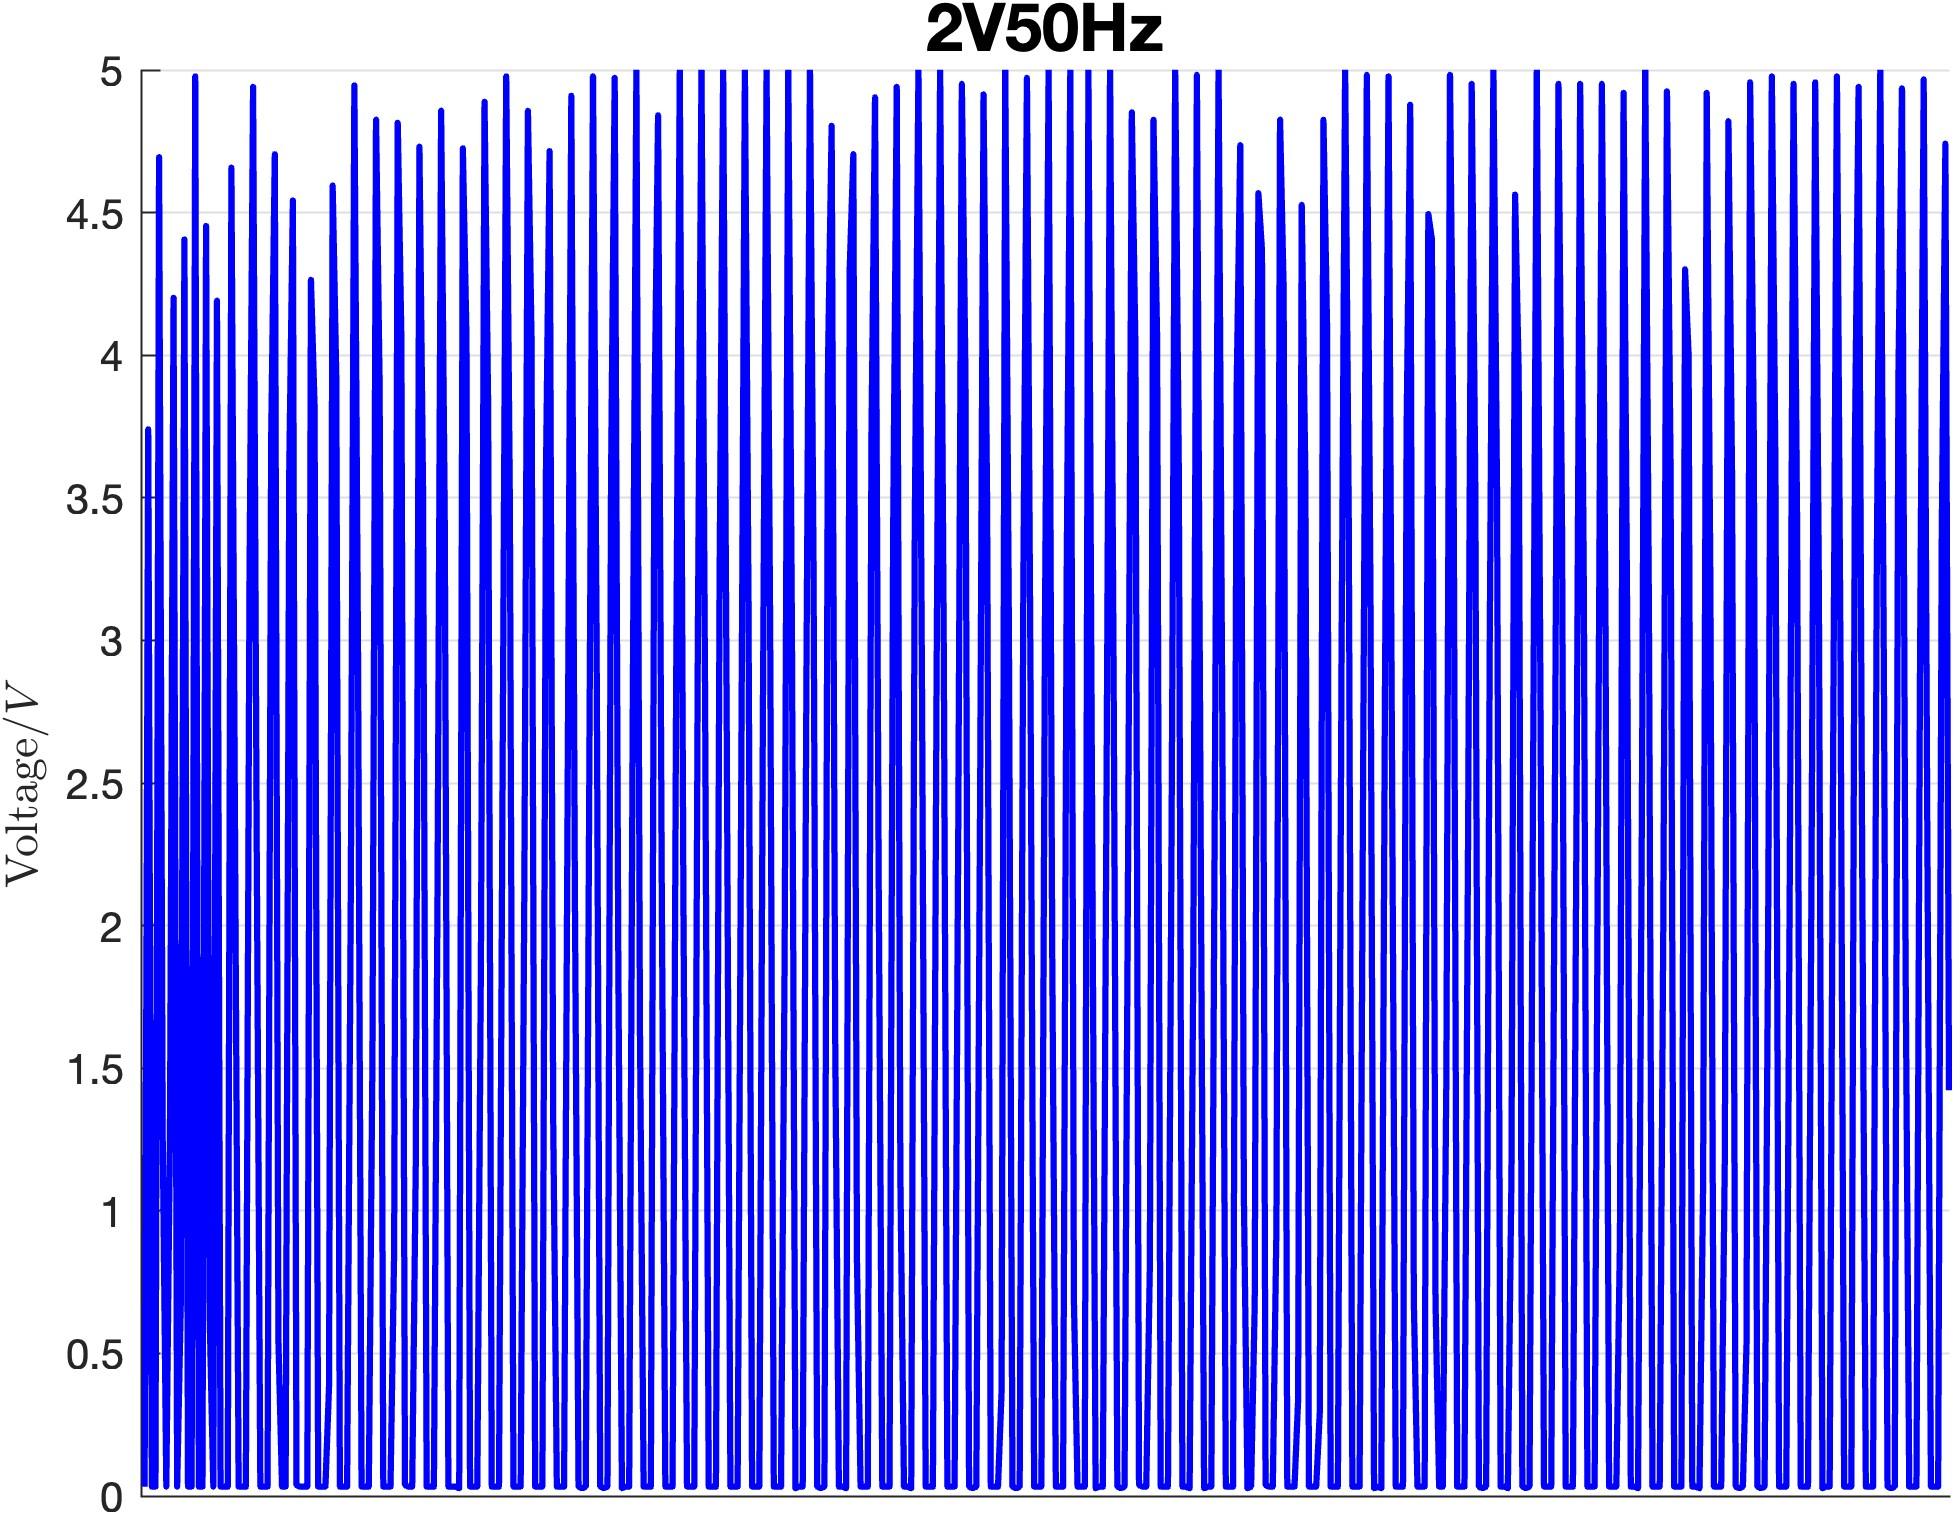
\includegraphics[width=\textwidth]{2V50Hz.jpg}
            \end{minipage}
            \\[3mm]
            \begin{minipage}[t]{0.32\textwidth}
                \centering
                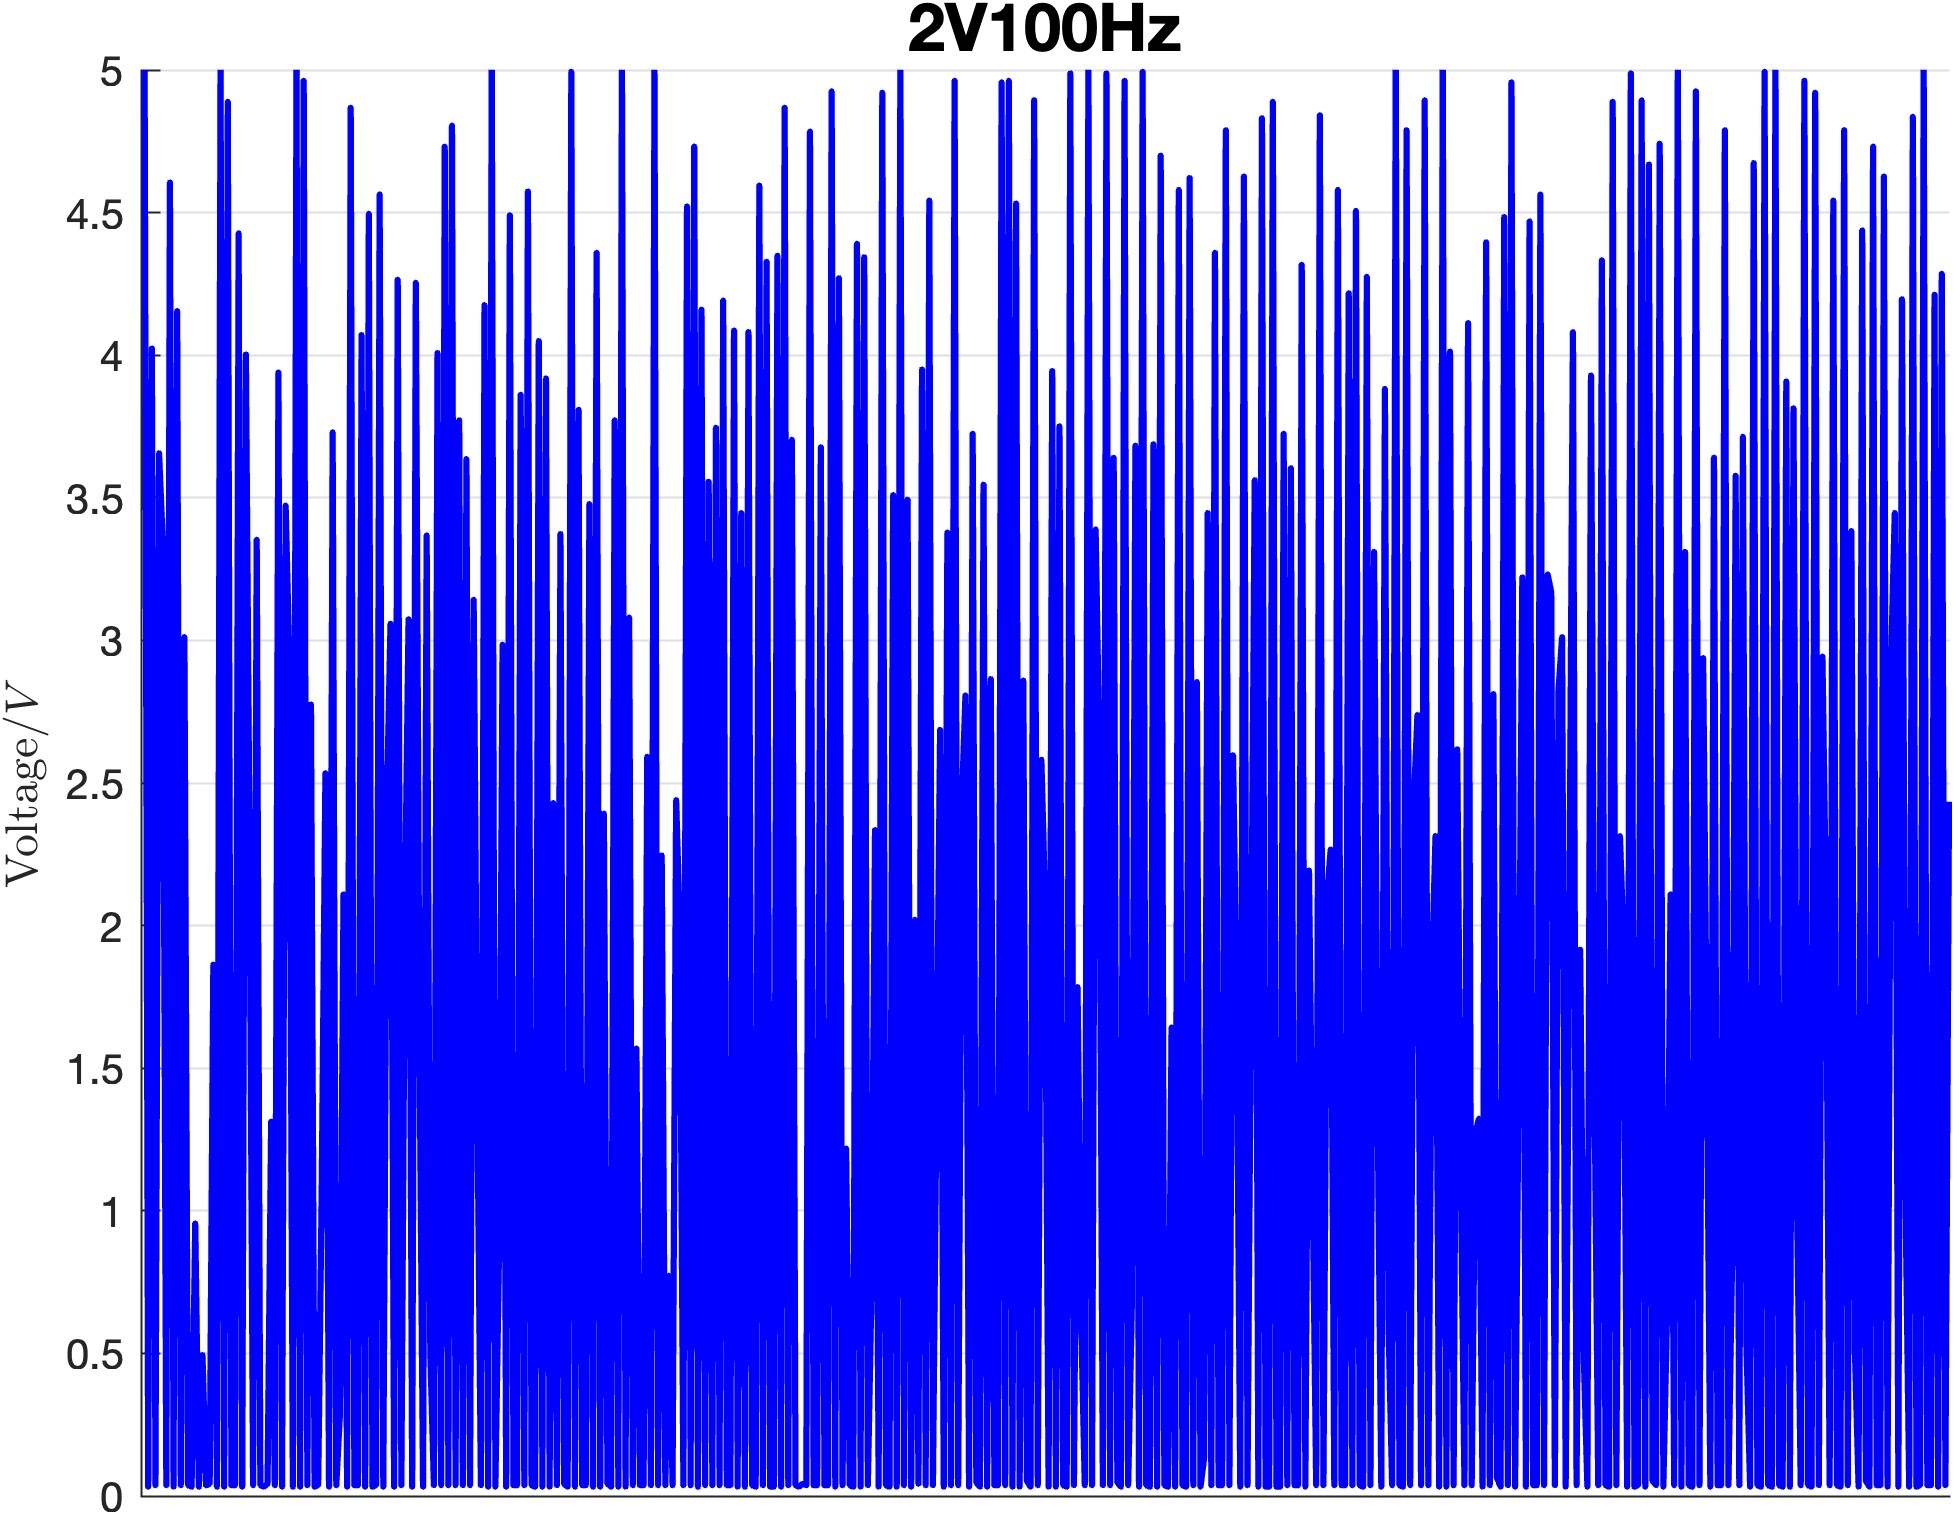
\includegraphics[width=\textwidth]{2V100Hz.jpg}
            \end{minipage}
            %\hfill
            \begin{minipage}[t]{0.32\textwidth}
                \centering
                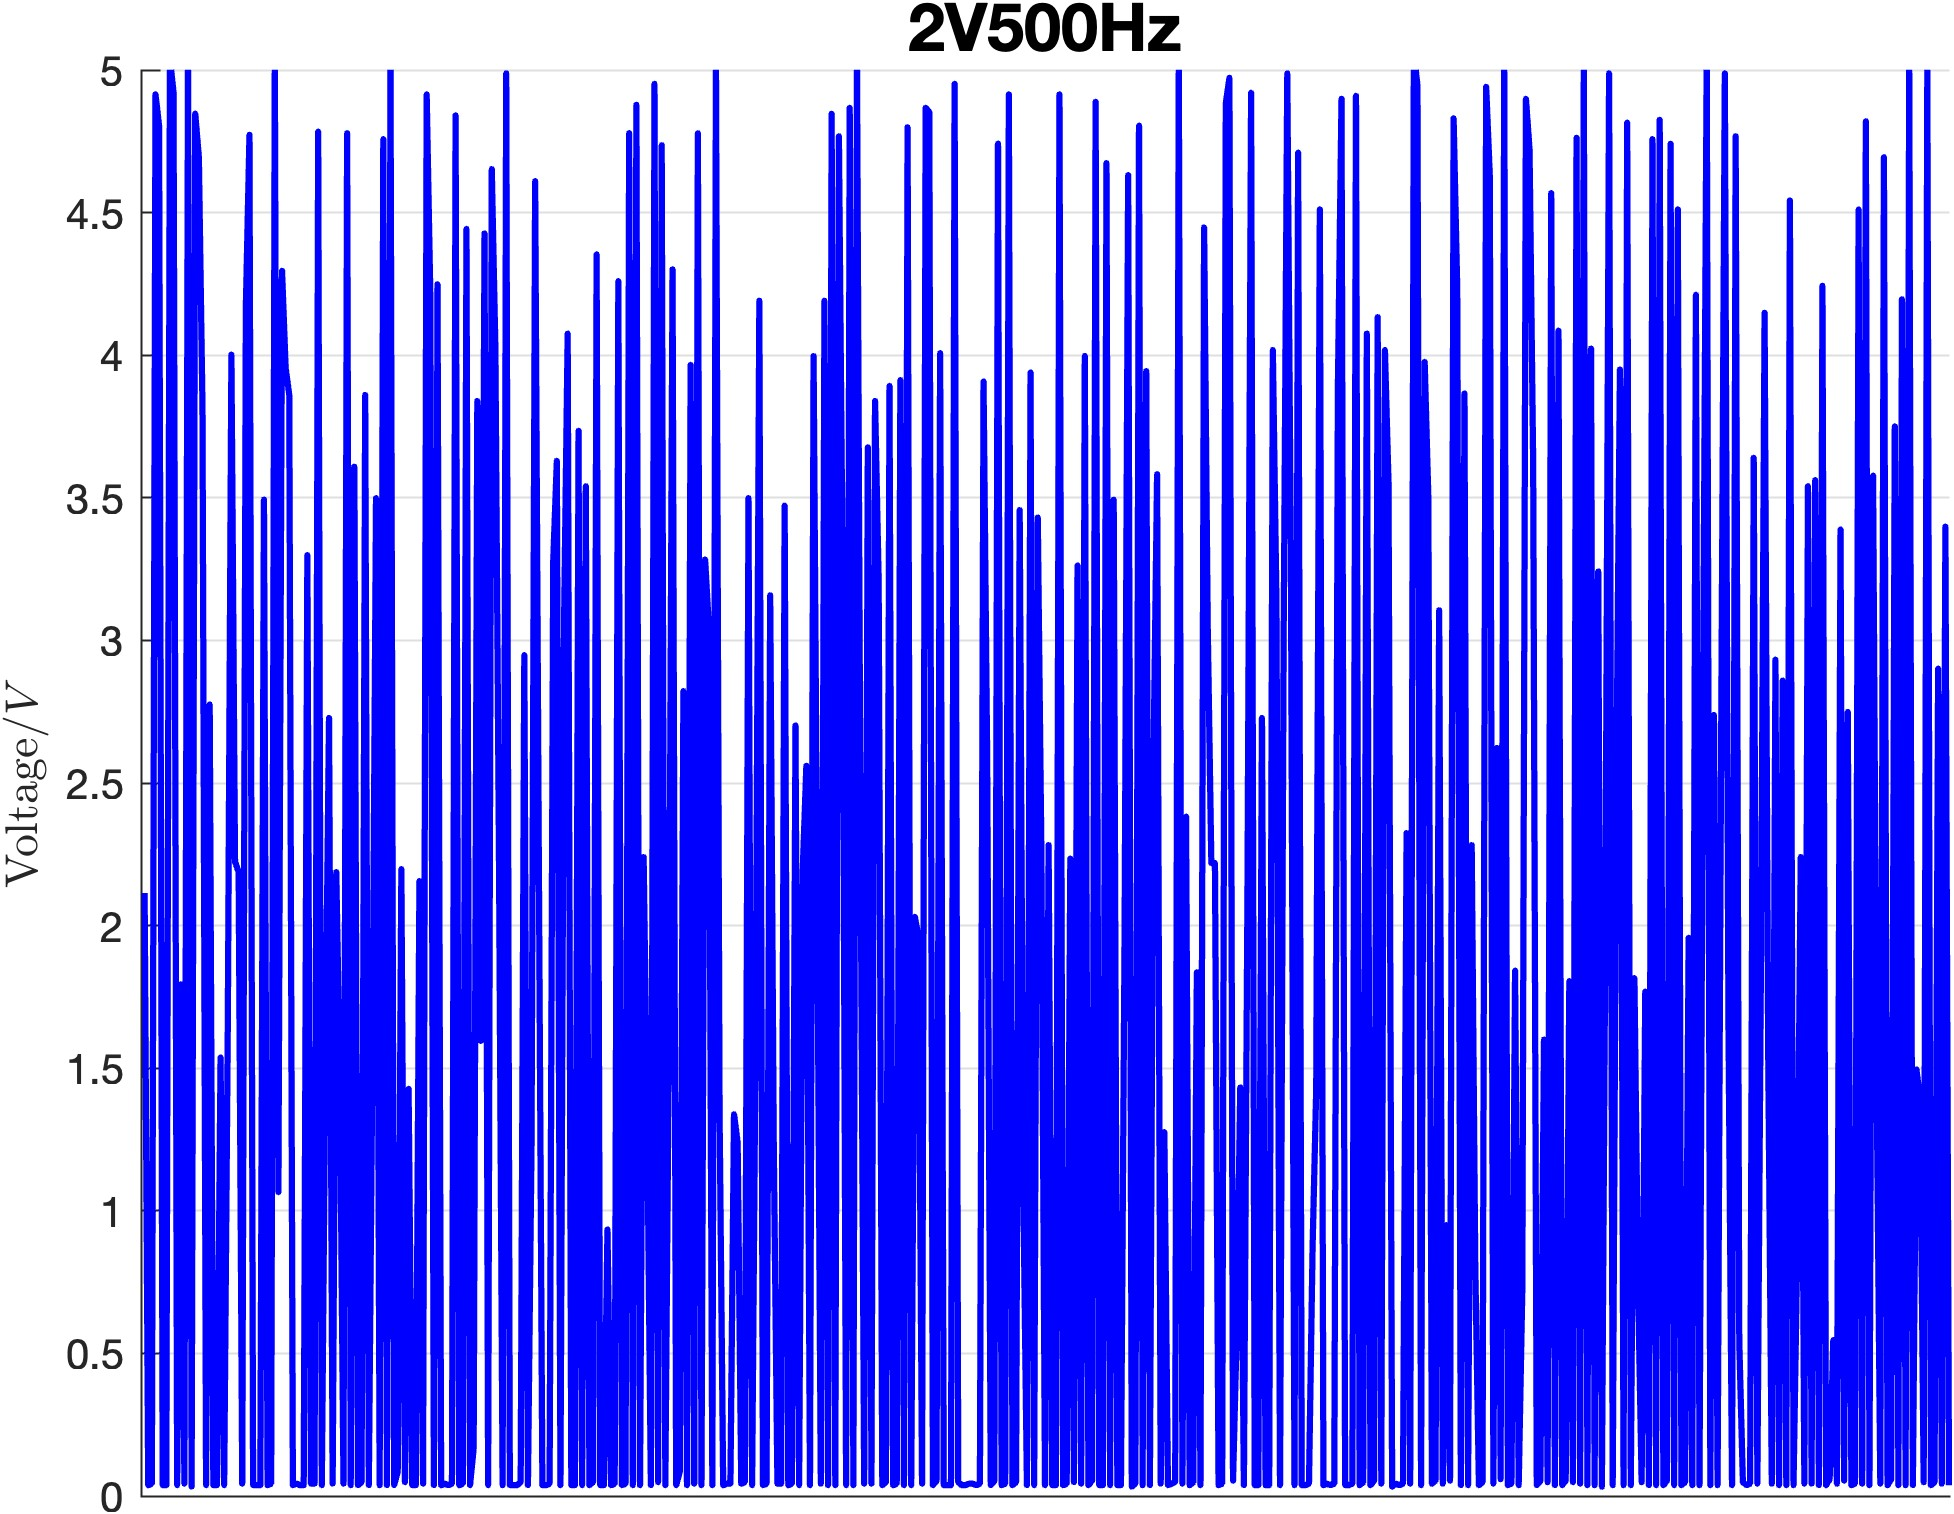
\includegraphics[width=\textwidth]{2V500Hz.jpg}
            \end{minipage}
            %\hfill
            \begin{minipage}[t]{0.32\textwidth}
                \centering
                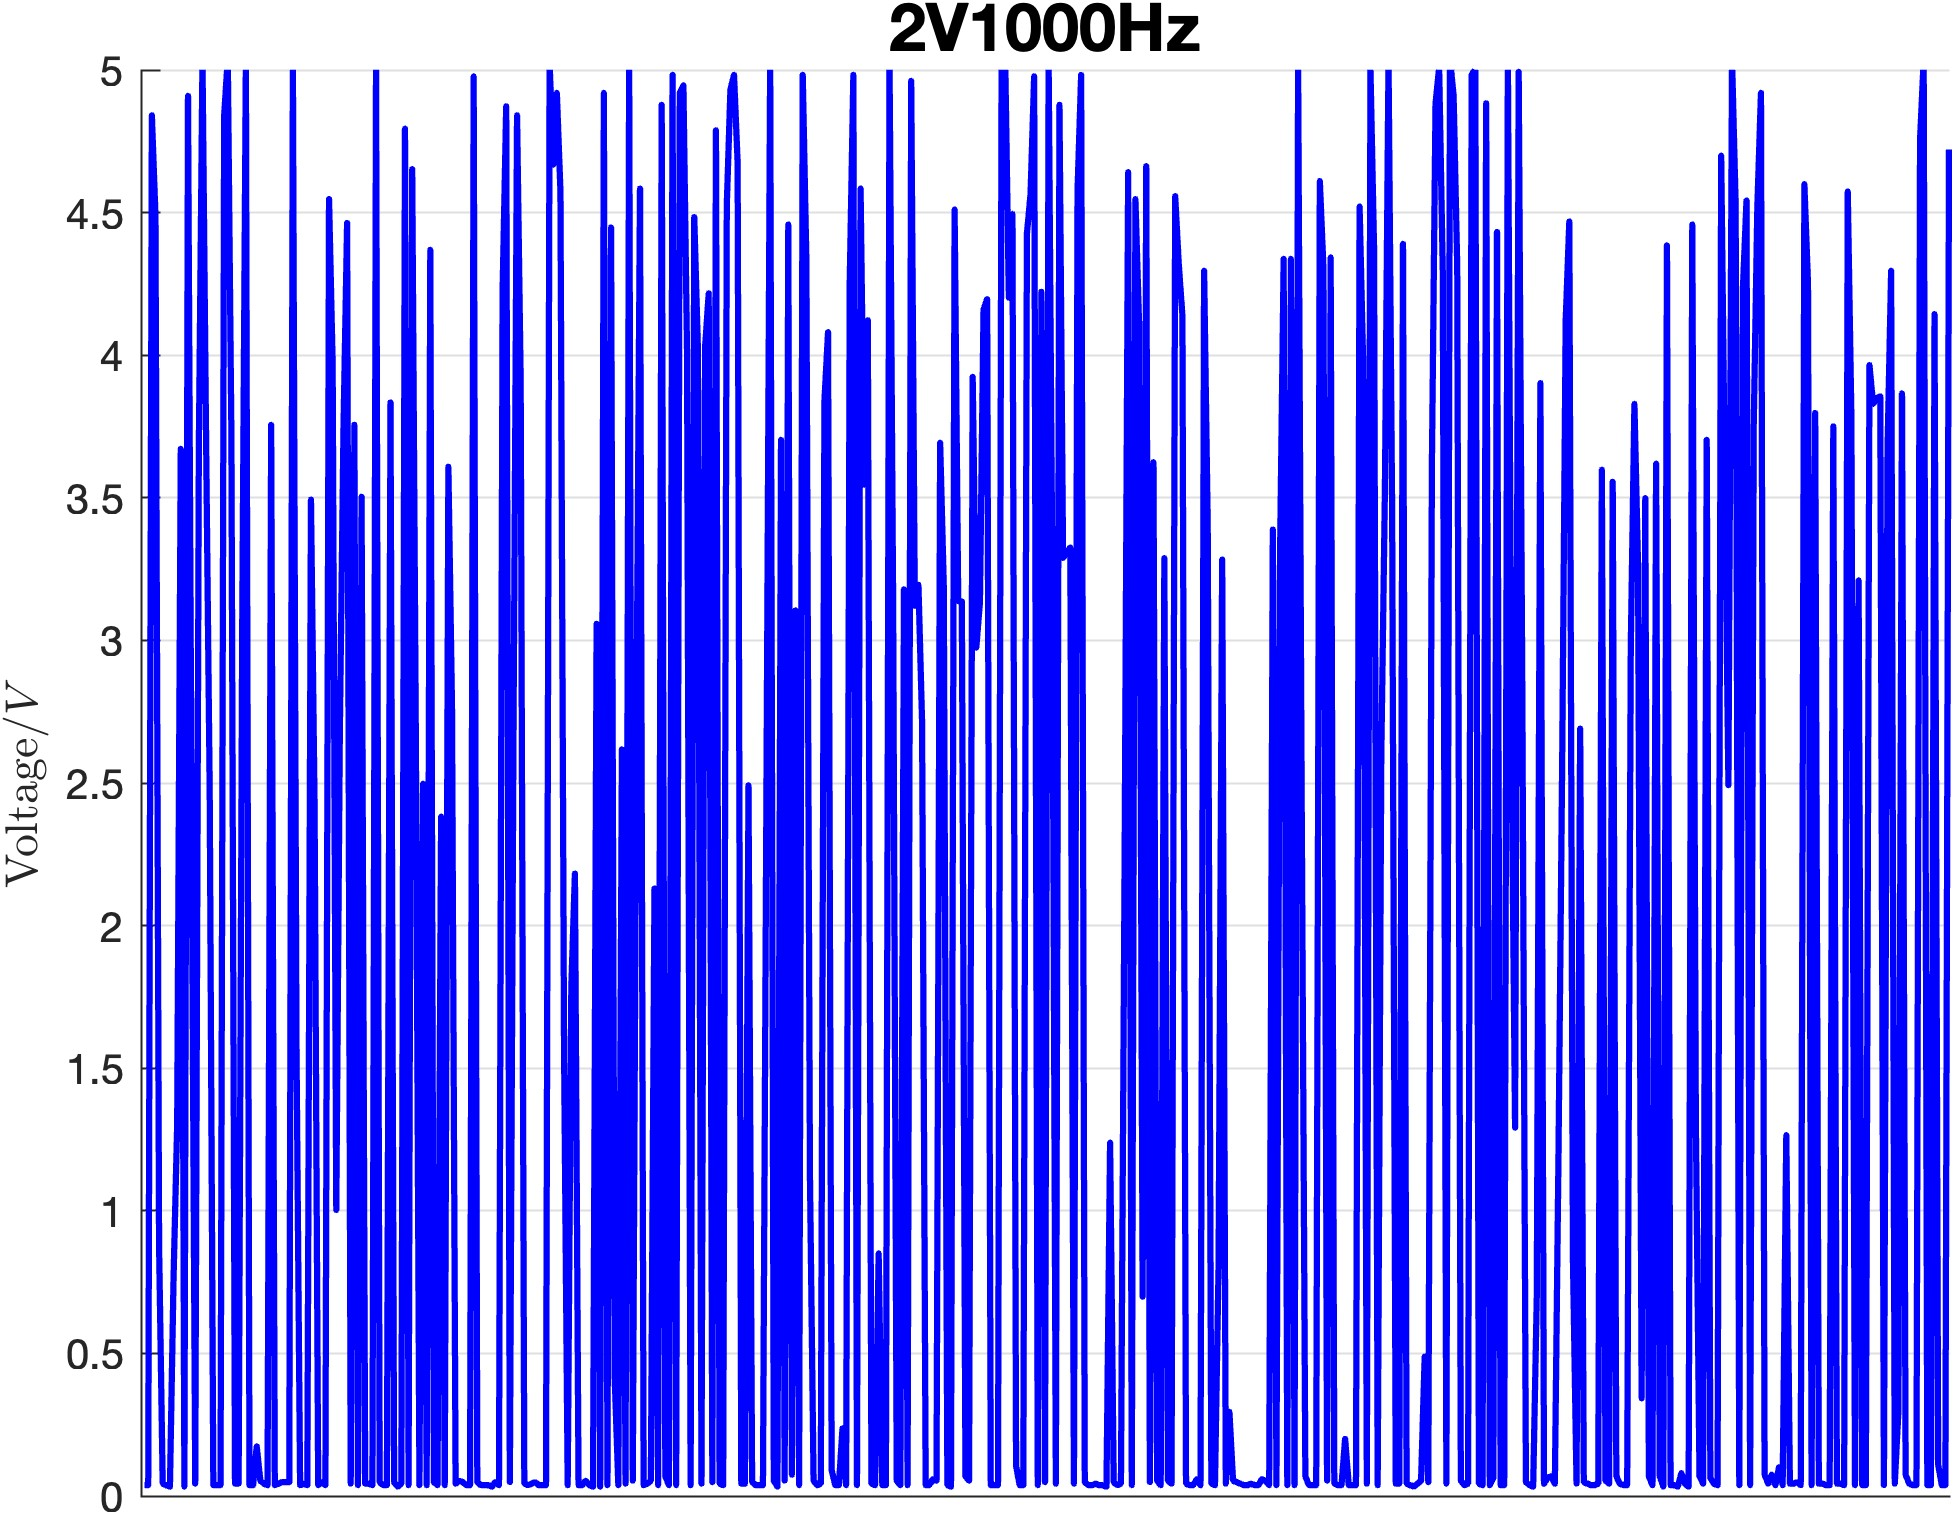
\includegraphics[width=\textwidth]{2V1000Hz.jpg}
            \end{minipage}
            \captionof{figure}{不同输入频率比较}
            \label{diffFreq}
        \end{minipage}
        \\[3mm]
        移除电路中的负反馈电容，重复上述频率变化，记录PD电路 $V_\text{out}$曲线如图~\ref{diffFreqW}。理论上此电容会限制高频增益，抑制高频噪声与震荡，并提供低通滤波作用，截止频率约为$f_c = 1/2\pi RC \approx \qty{21.2}{\Hz}$。然而实际测量的图像基本保持一致，电容并未起到滤波的作用，其原因可能为：对高频信号$\qty{0.1}{\uF}$的阻抗非常低，几乎等于电流短路走电容，输出电压反而保持了原来的快速响应，滤波效果形同虚设；另外NI DAQ的最快信号捕获频率也有可能限制了波形的显示。
        \\[6mm]
        \begin{minipage}{\linewidth}    
            \centering
            \begin{minipage}[t]{0.32\textwidth}
                \centering
                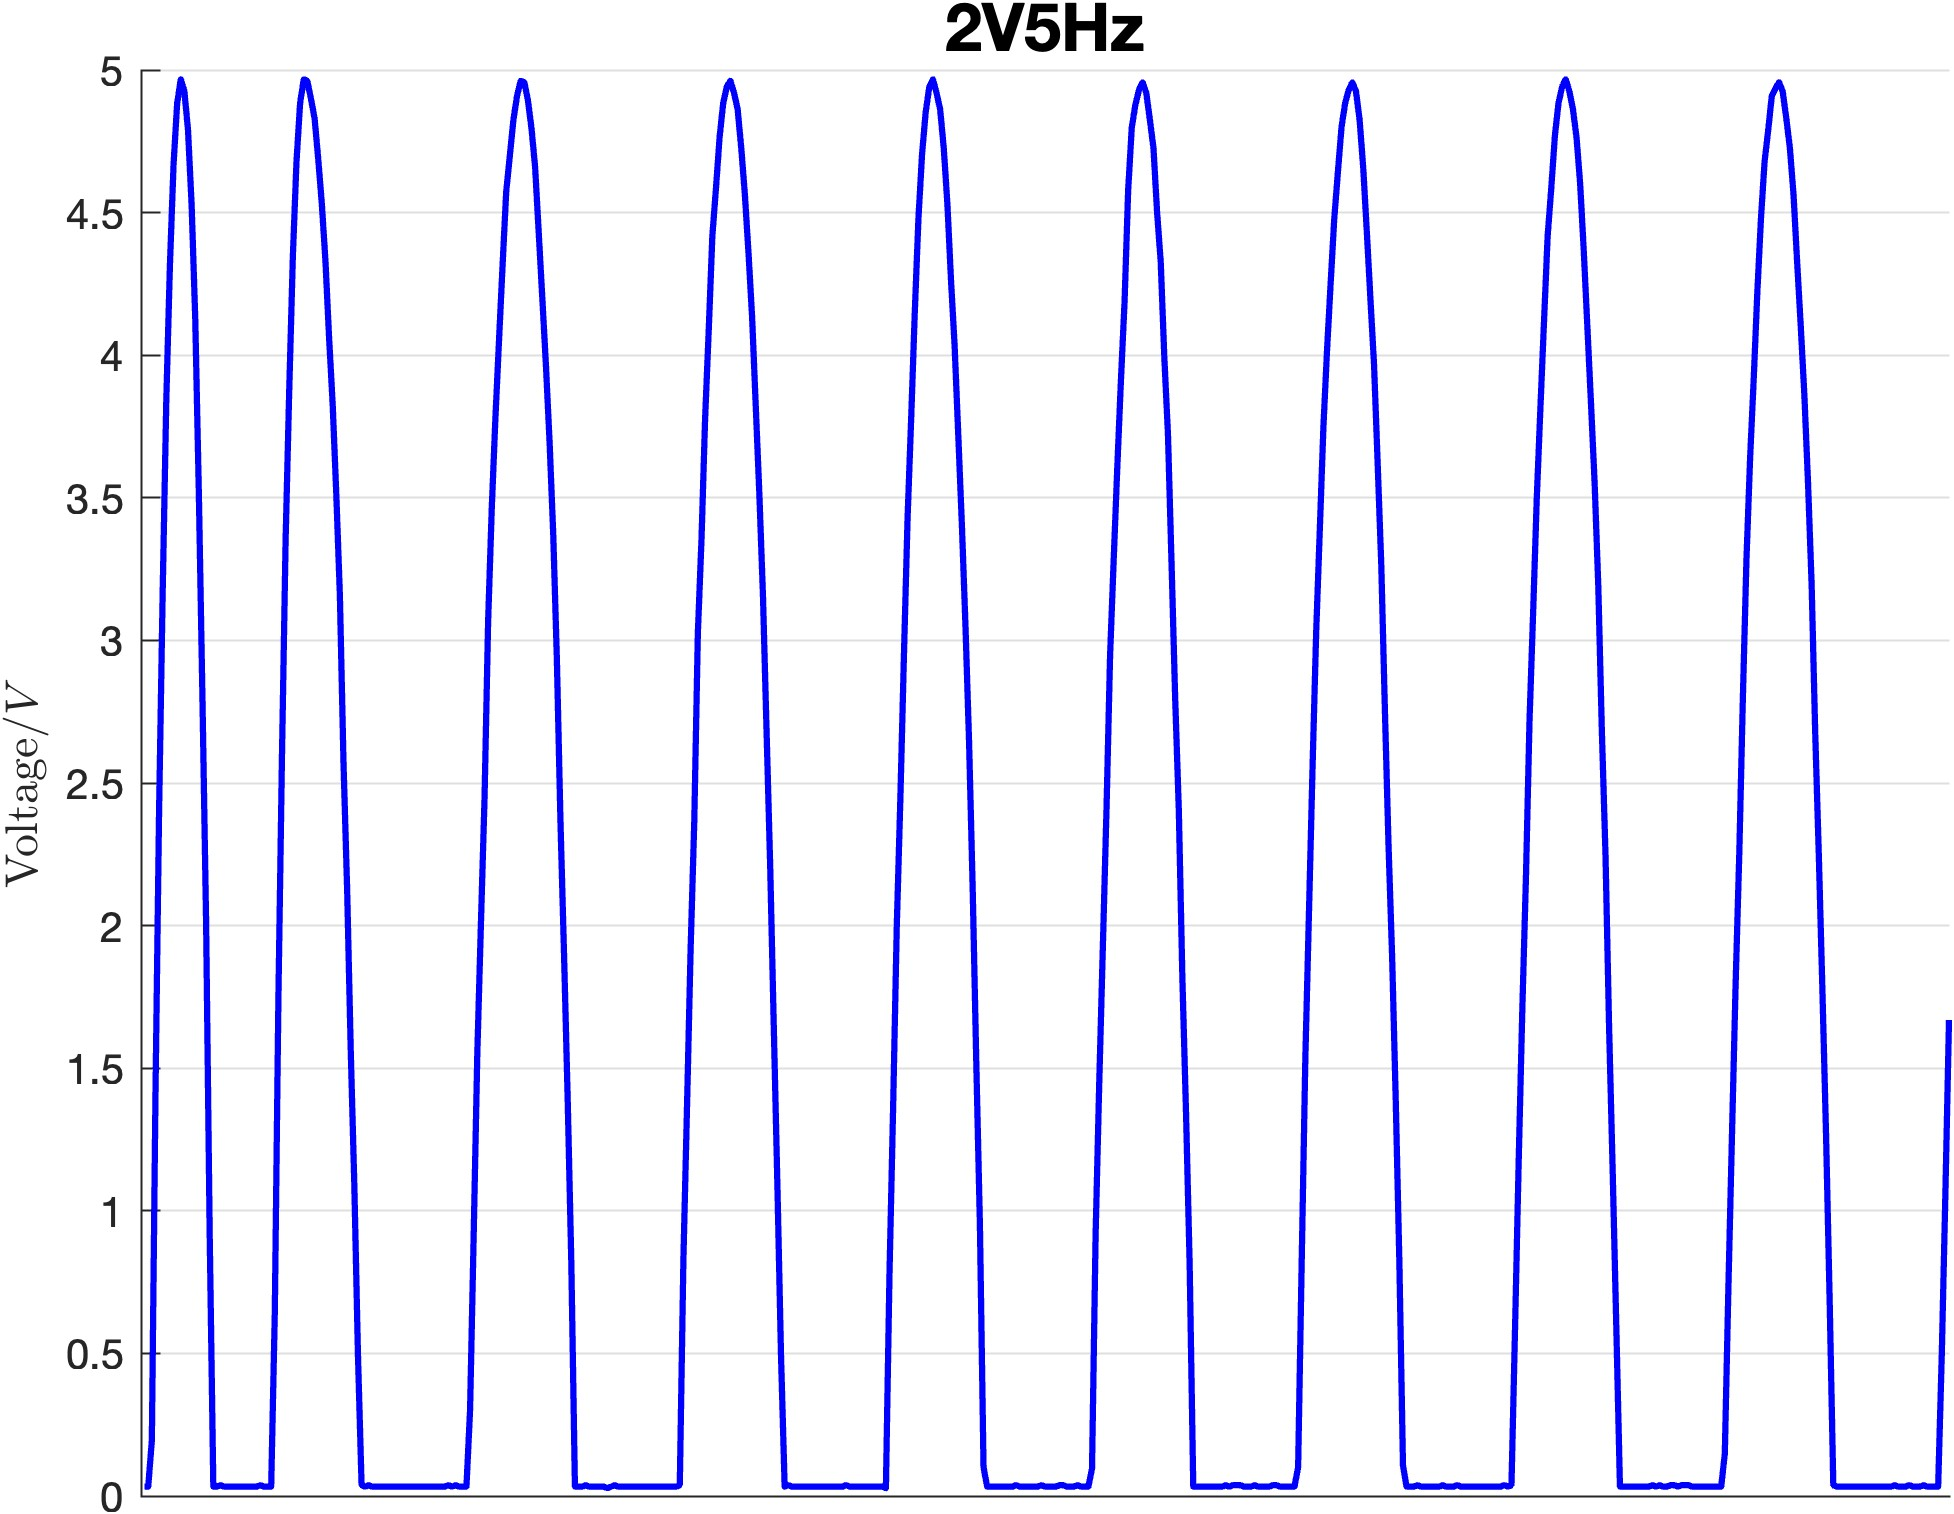
\includegraphics[width=\textwidth]{2V5HzW.jpg}
            \end{minipage}
            %\hfill
            \begin{minipage}[t]{0.32\textwidth}
                \centering
                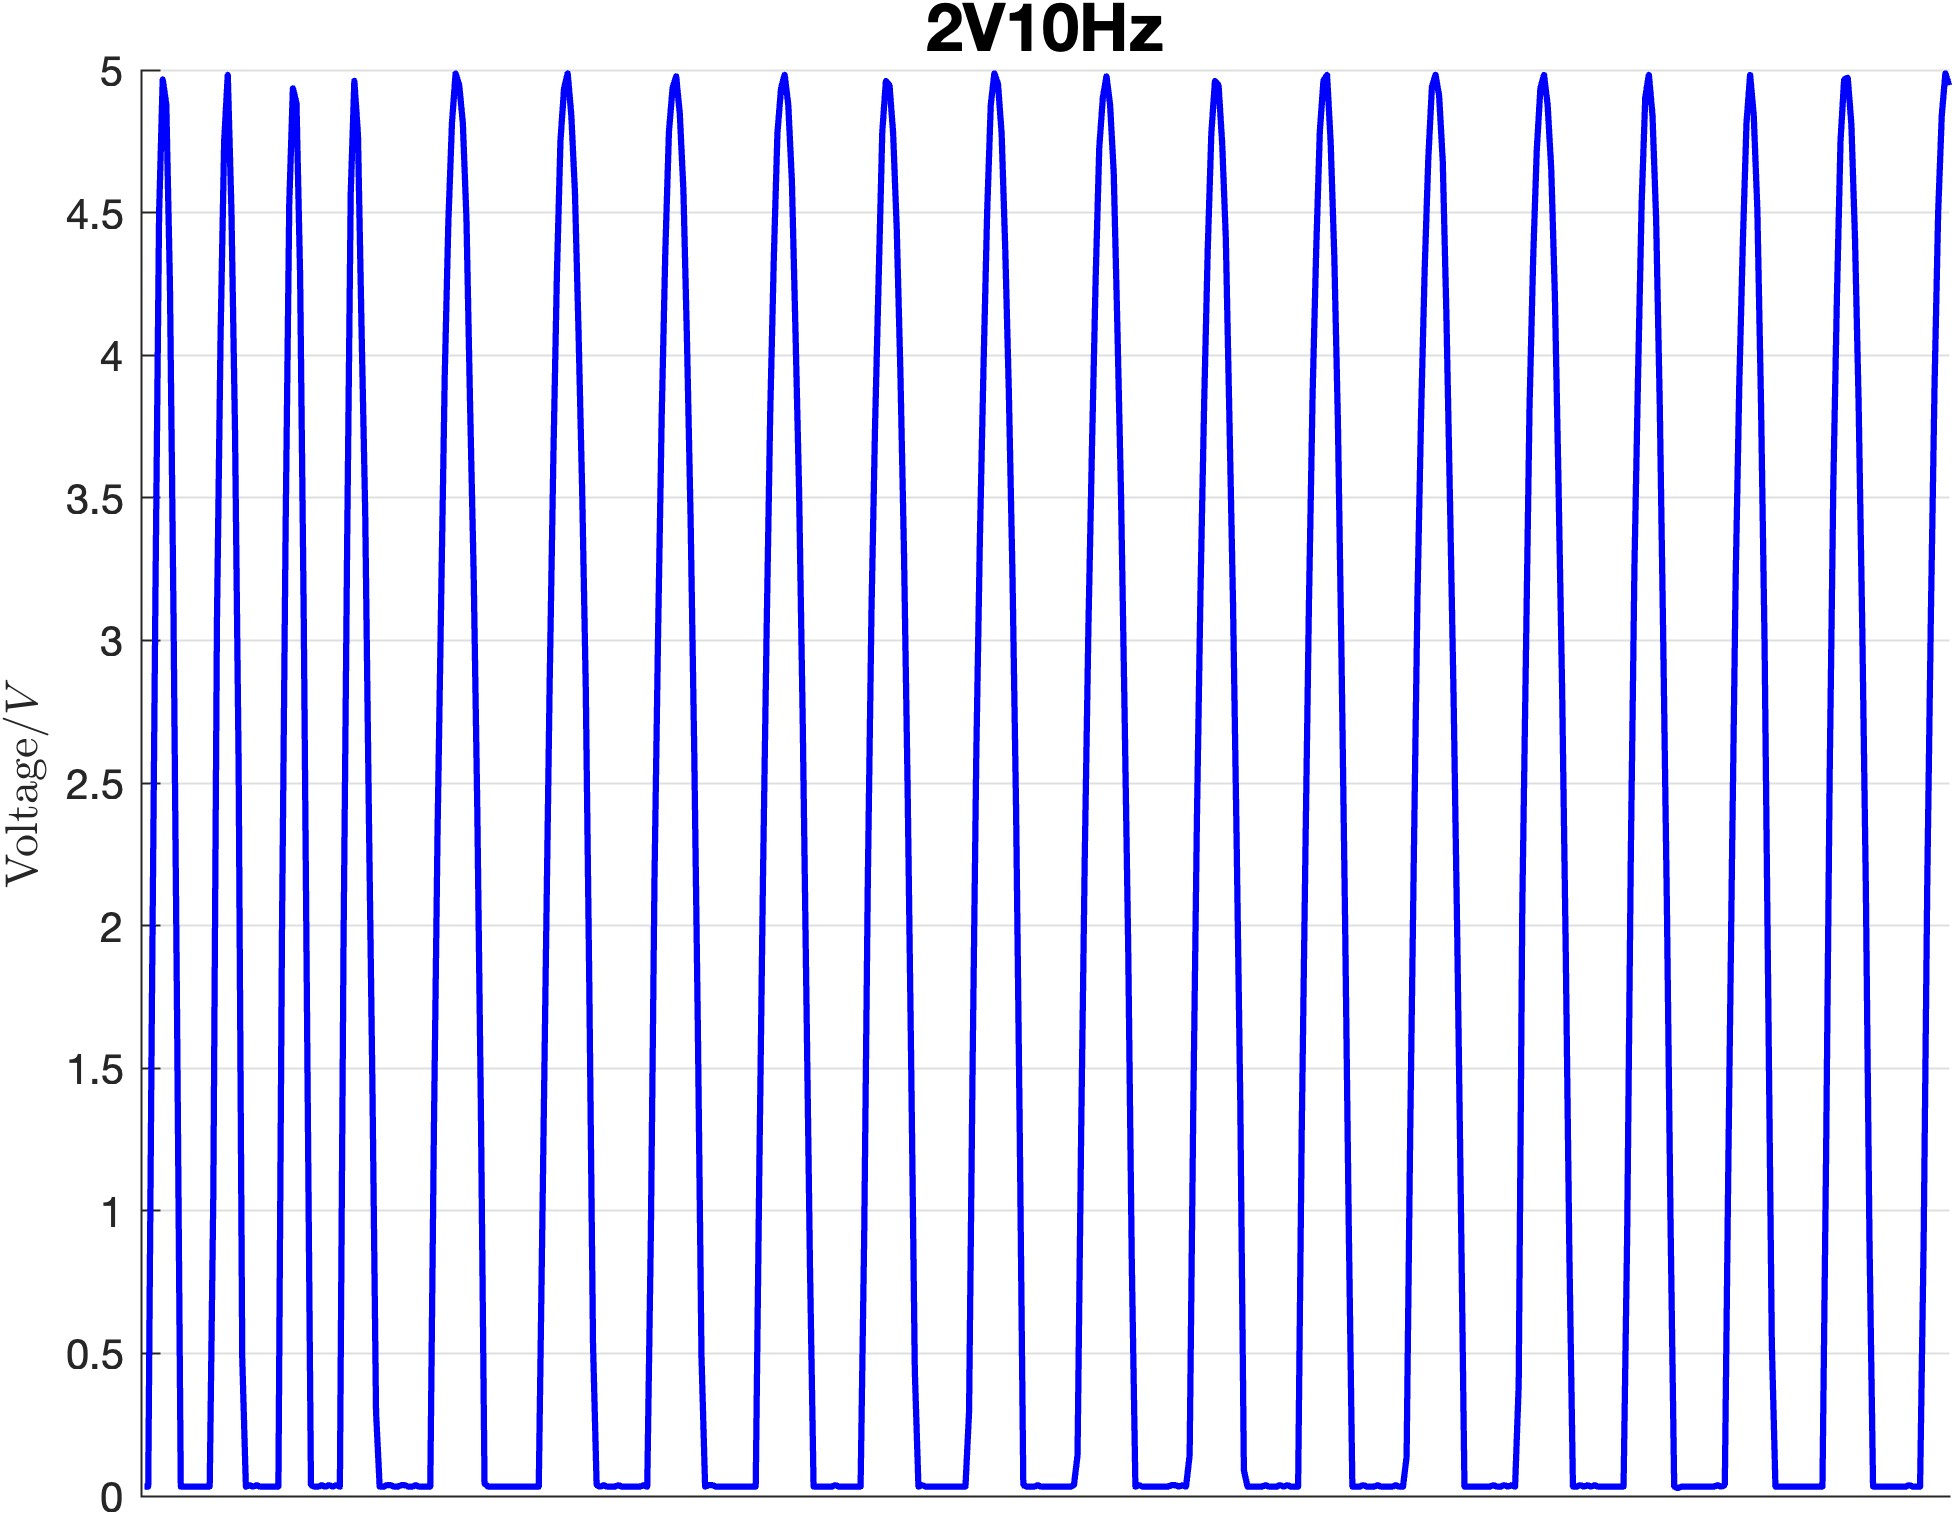
\includegraphics[width=\textwidth]{2V10HzW.jpg}
            \end{minipage}
            %\hfill
            \begin{minipage}[t]{0.32\textwidth}
                \centering
                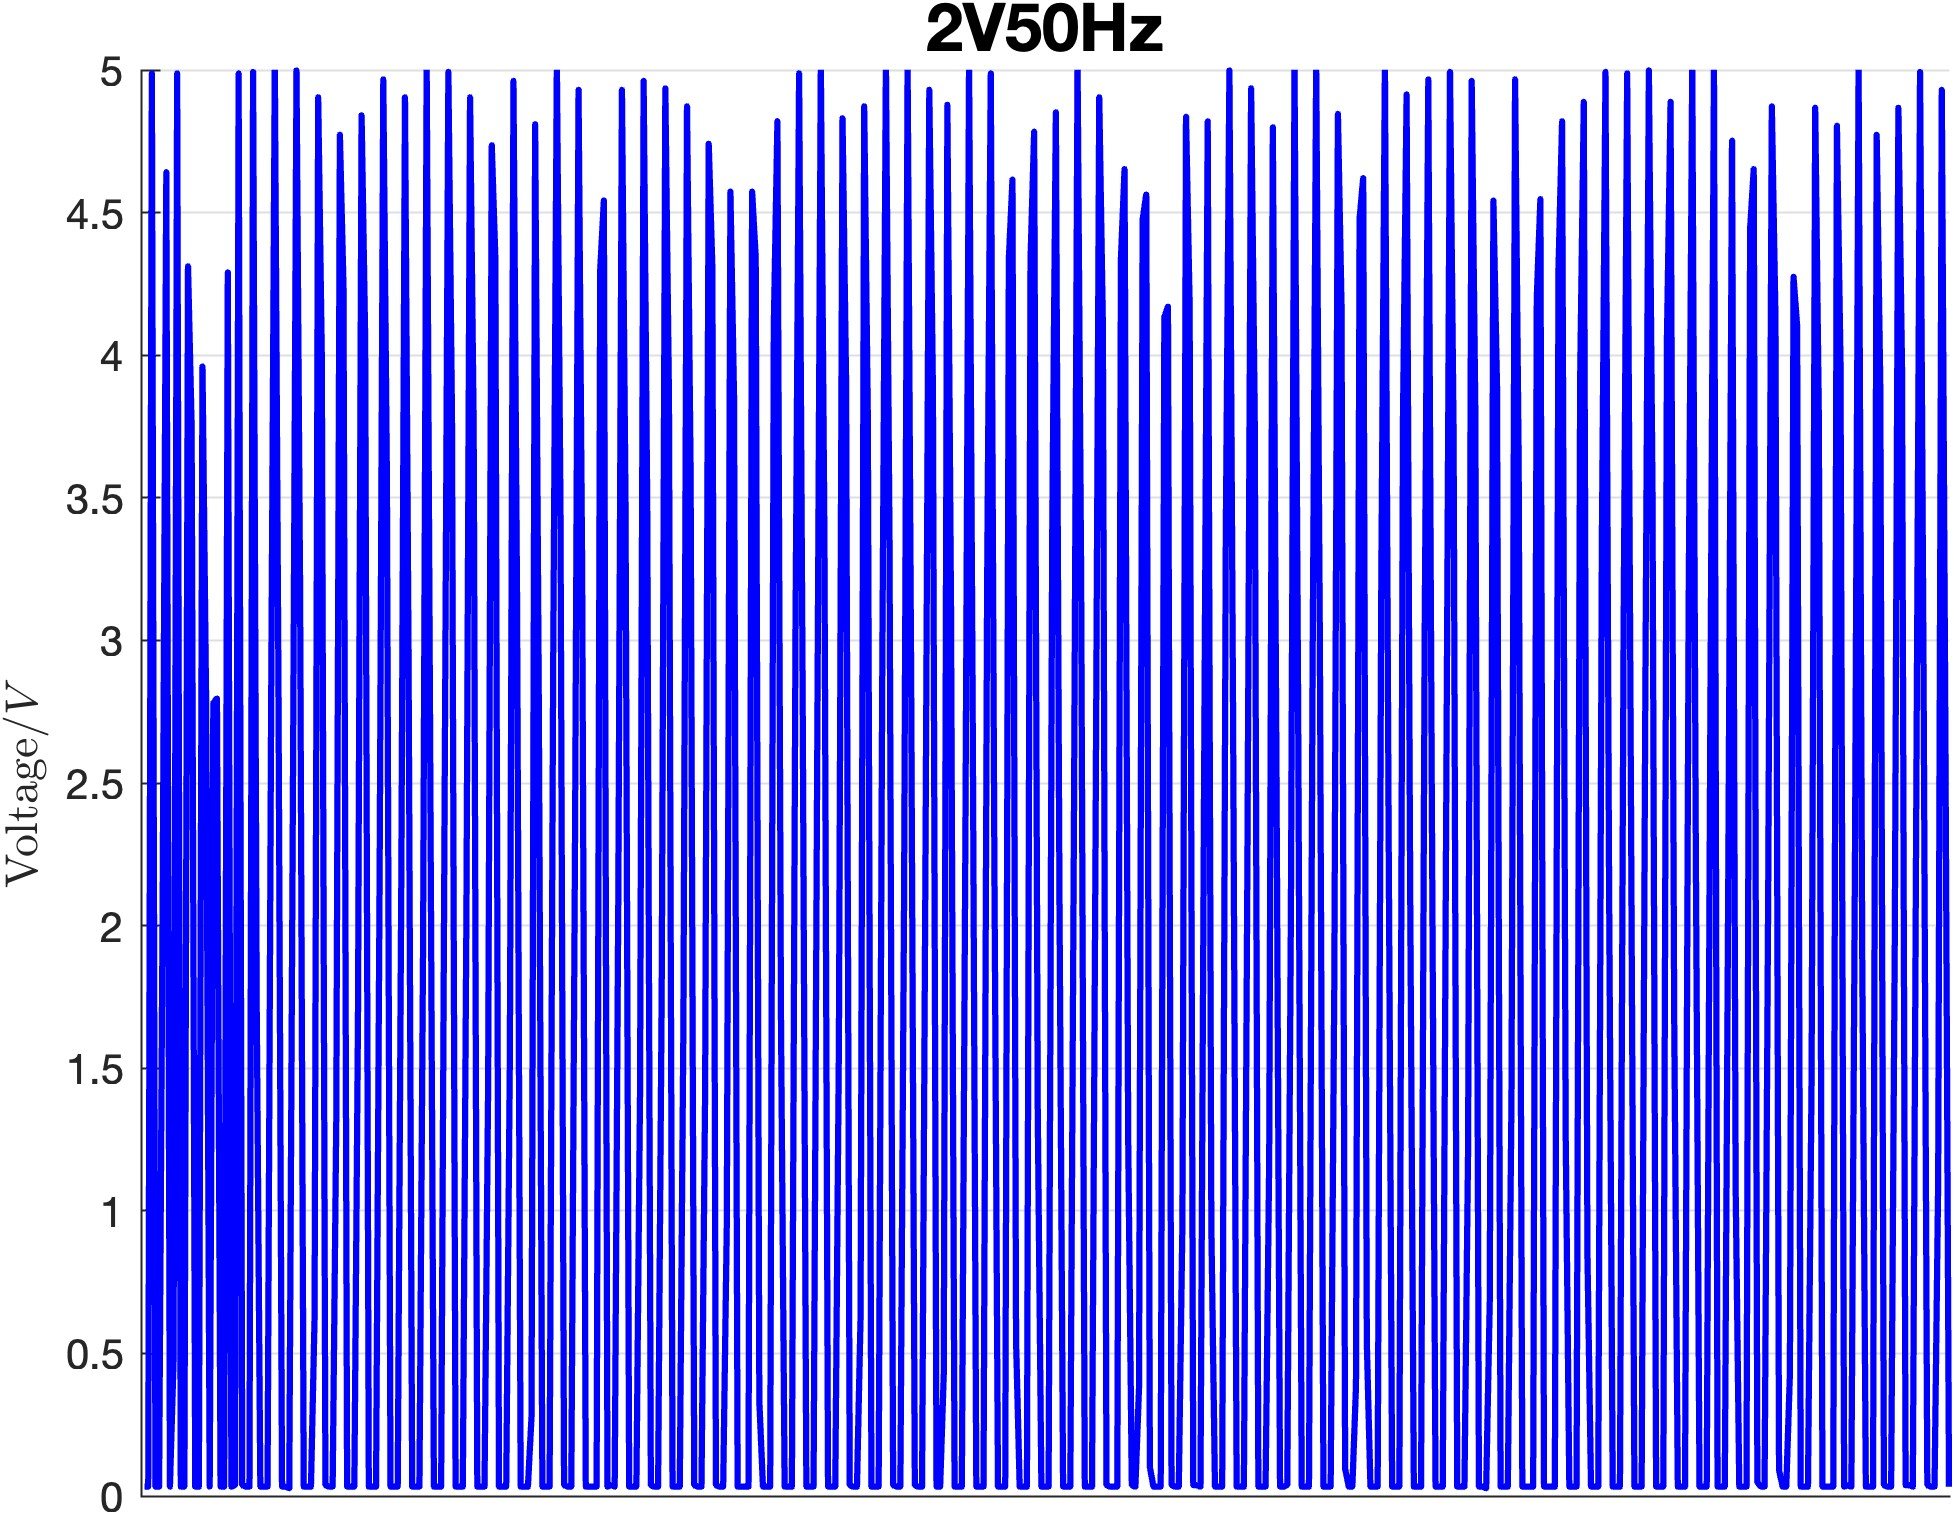
\includegraphics[width=\textwidth]{2V50HzW.jpg}
            \end{minipage}
        \end{minipage} 
        \begin{minipage}{\linewidth}    
            \begin{minipage}[t]{0.32\textwidth}
                \centering
                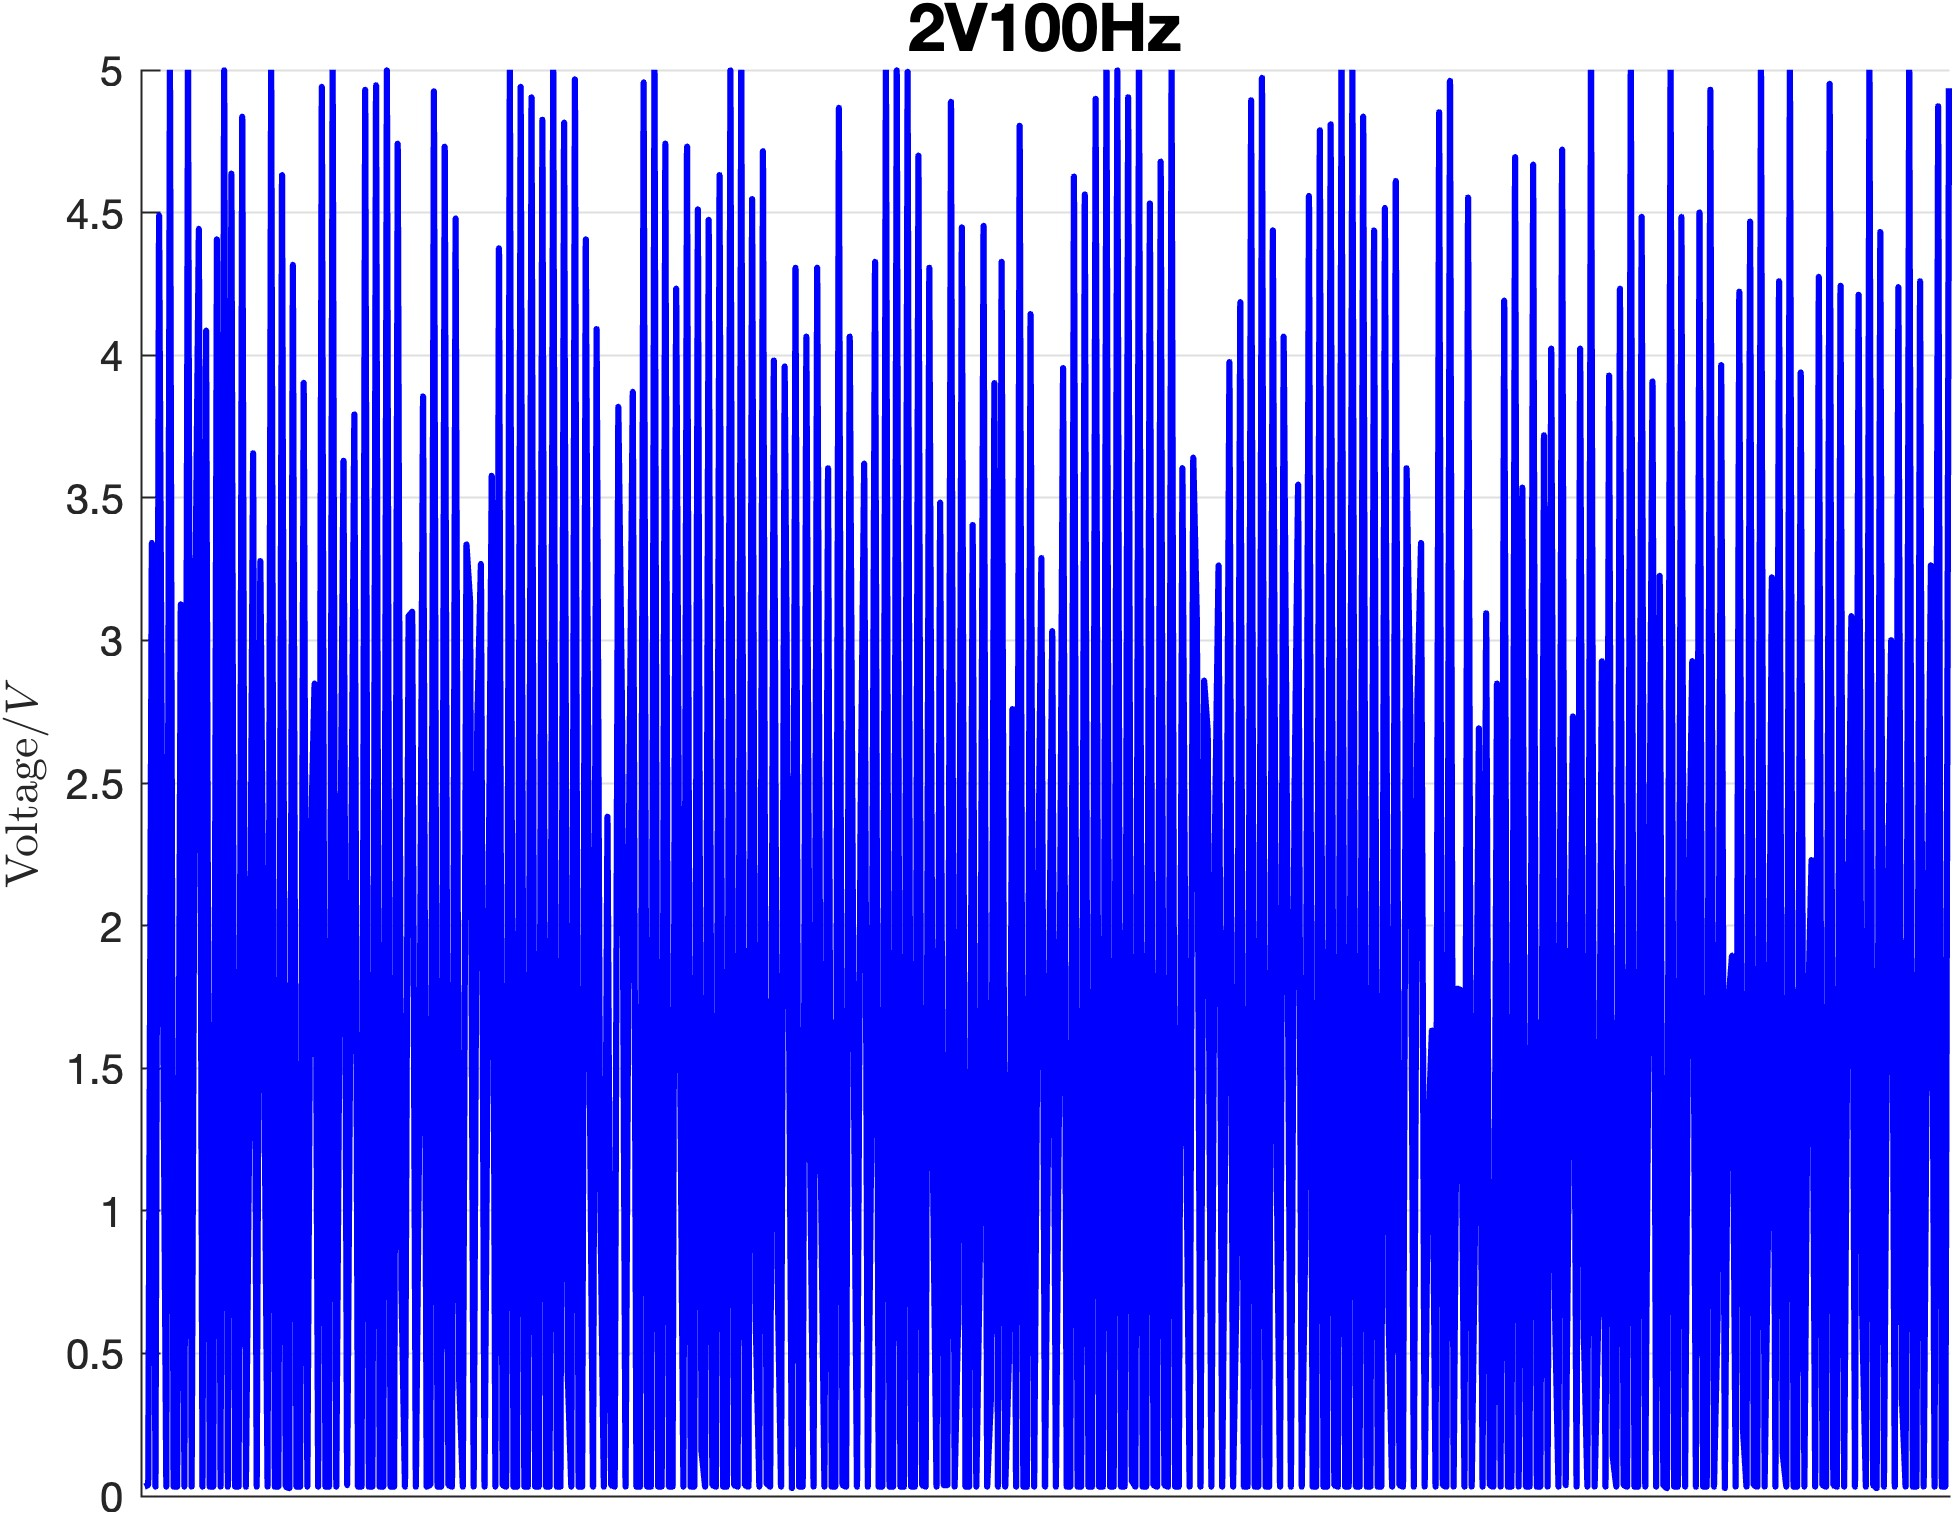
\includegraphics[width=\textwidth]{2V100HzW.jpg}
            \end{minipage}
            %\hfill
            \begin{minipage}[t]{0.32\textwidth}
                \centering
                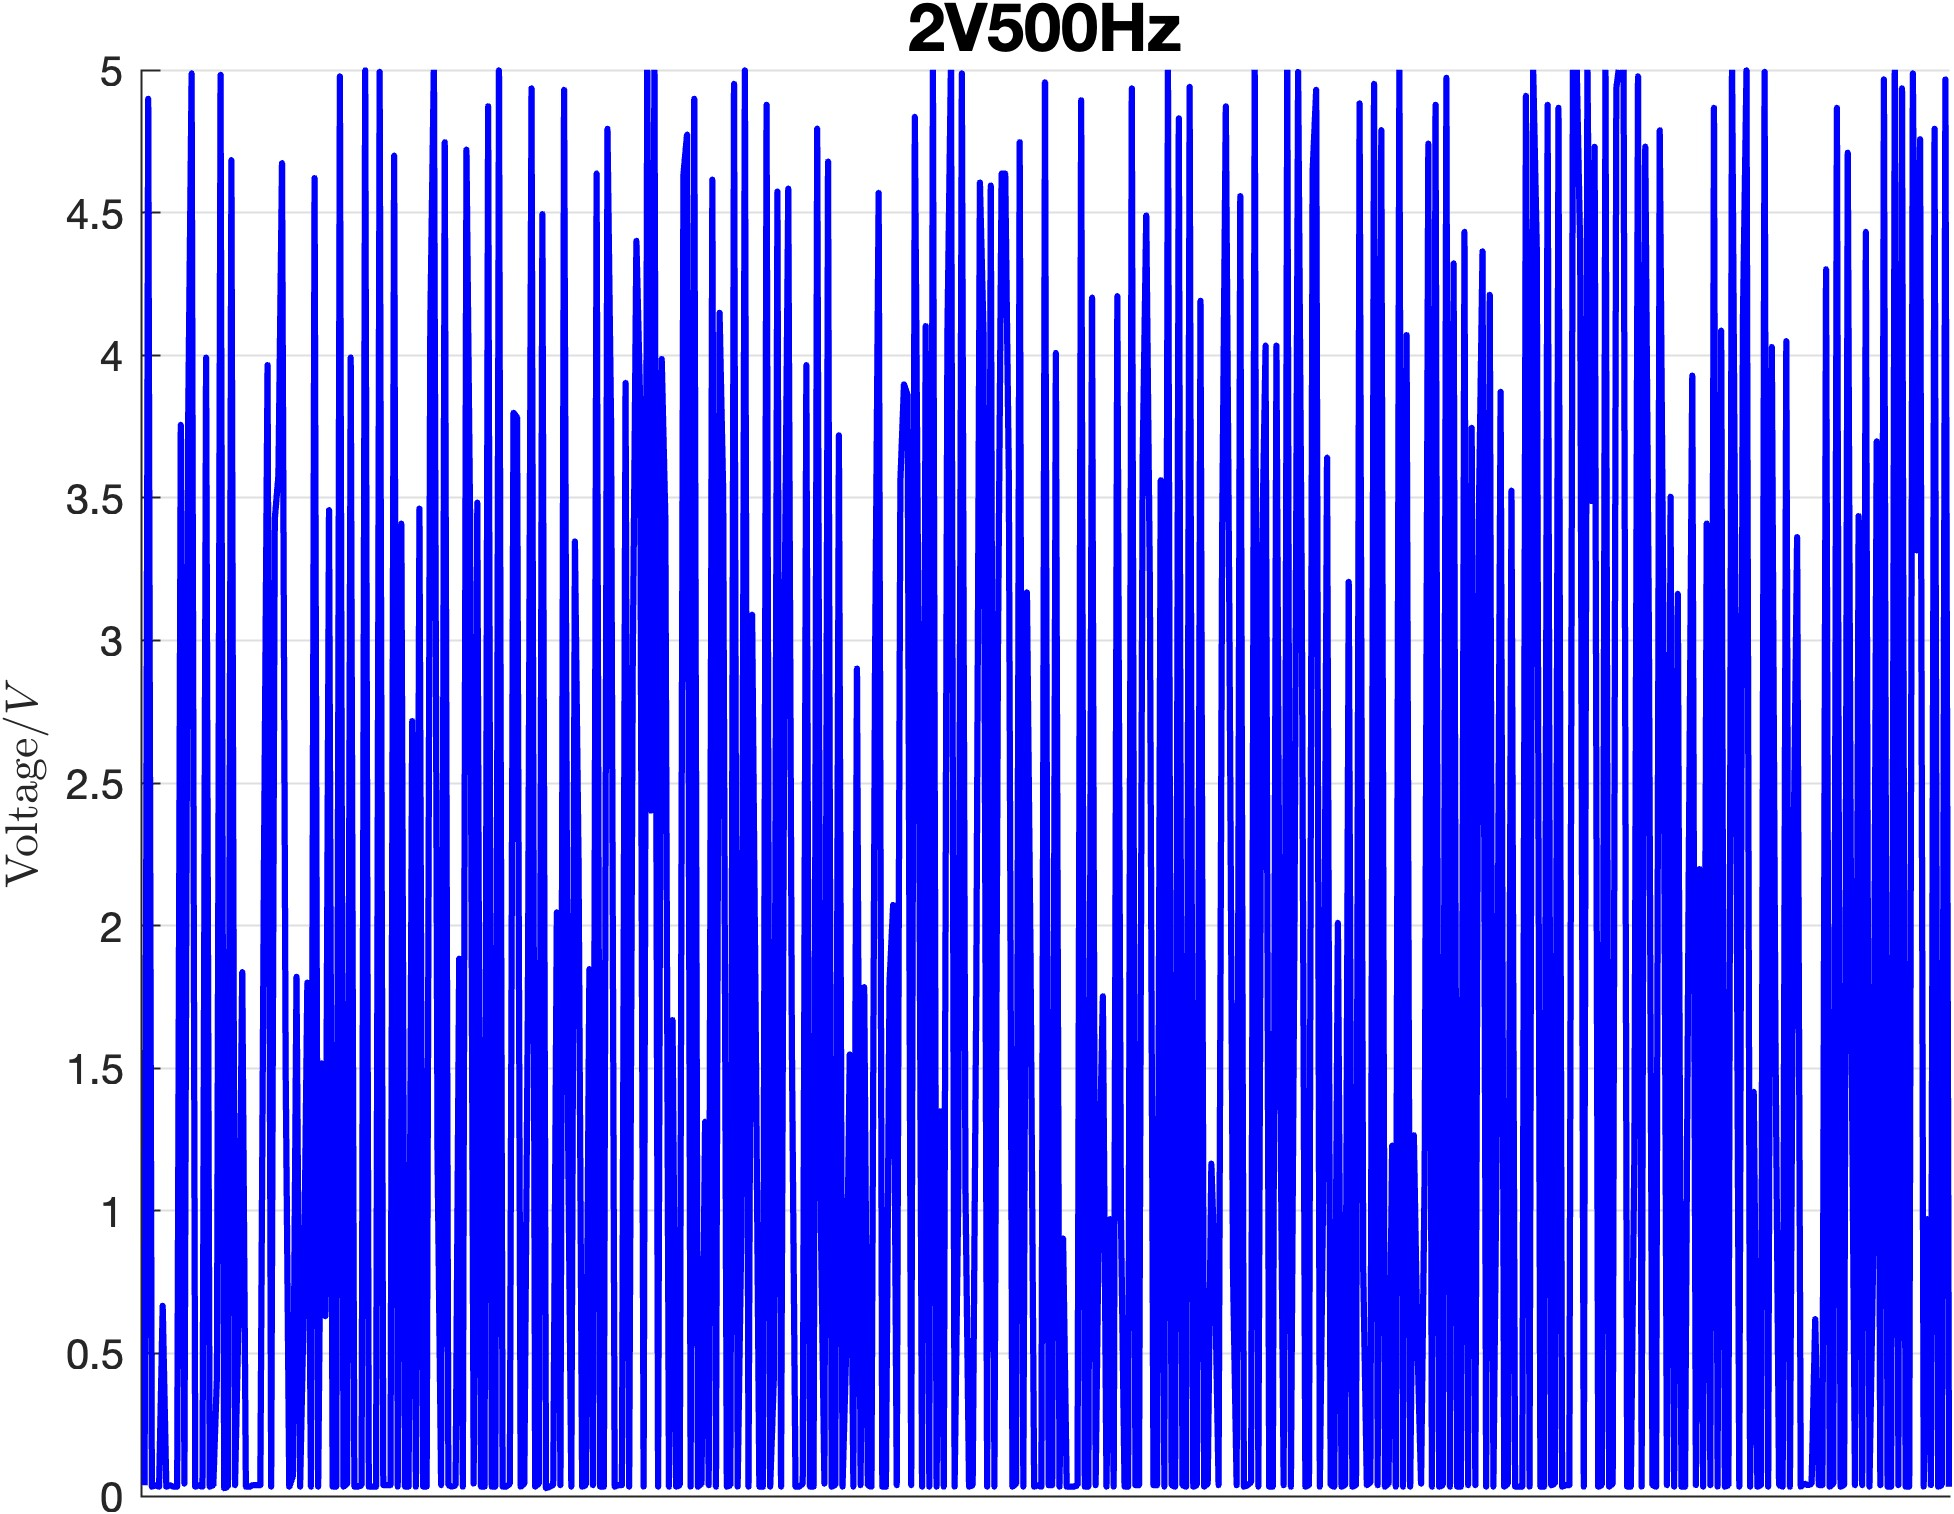
\includegraphics[width=\textwidth]{2V500HzW.jpg}
            \end{minipage}
            %\hfill
            \begin{minipage}[t]{0.32\textwidth}
                \centering
                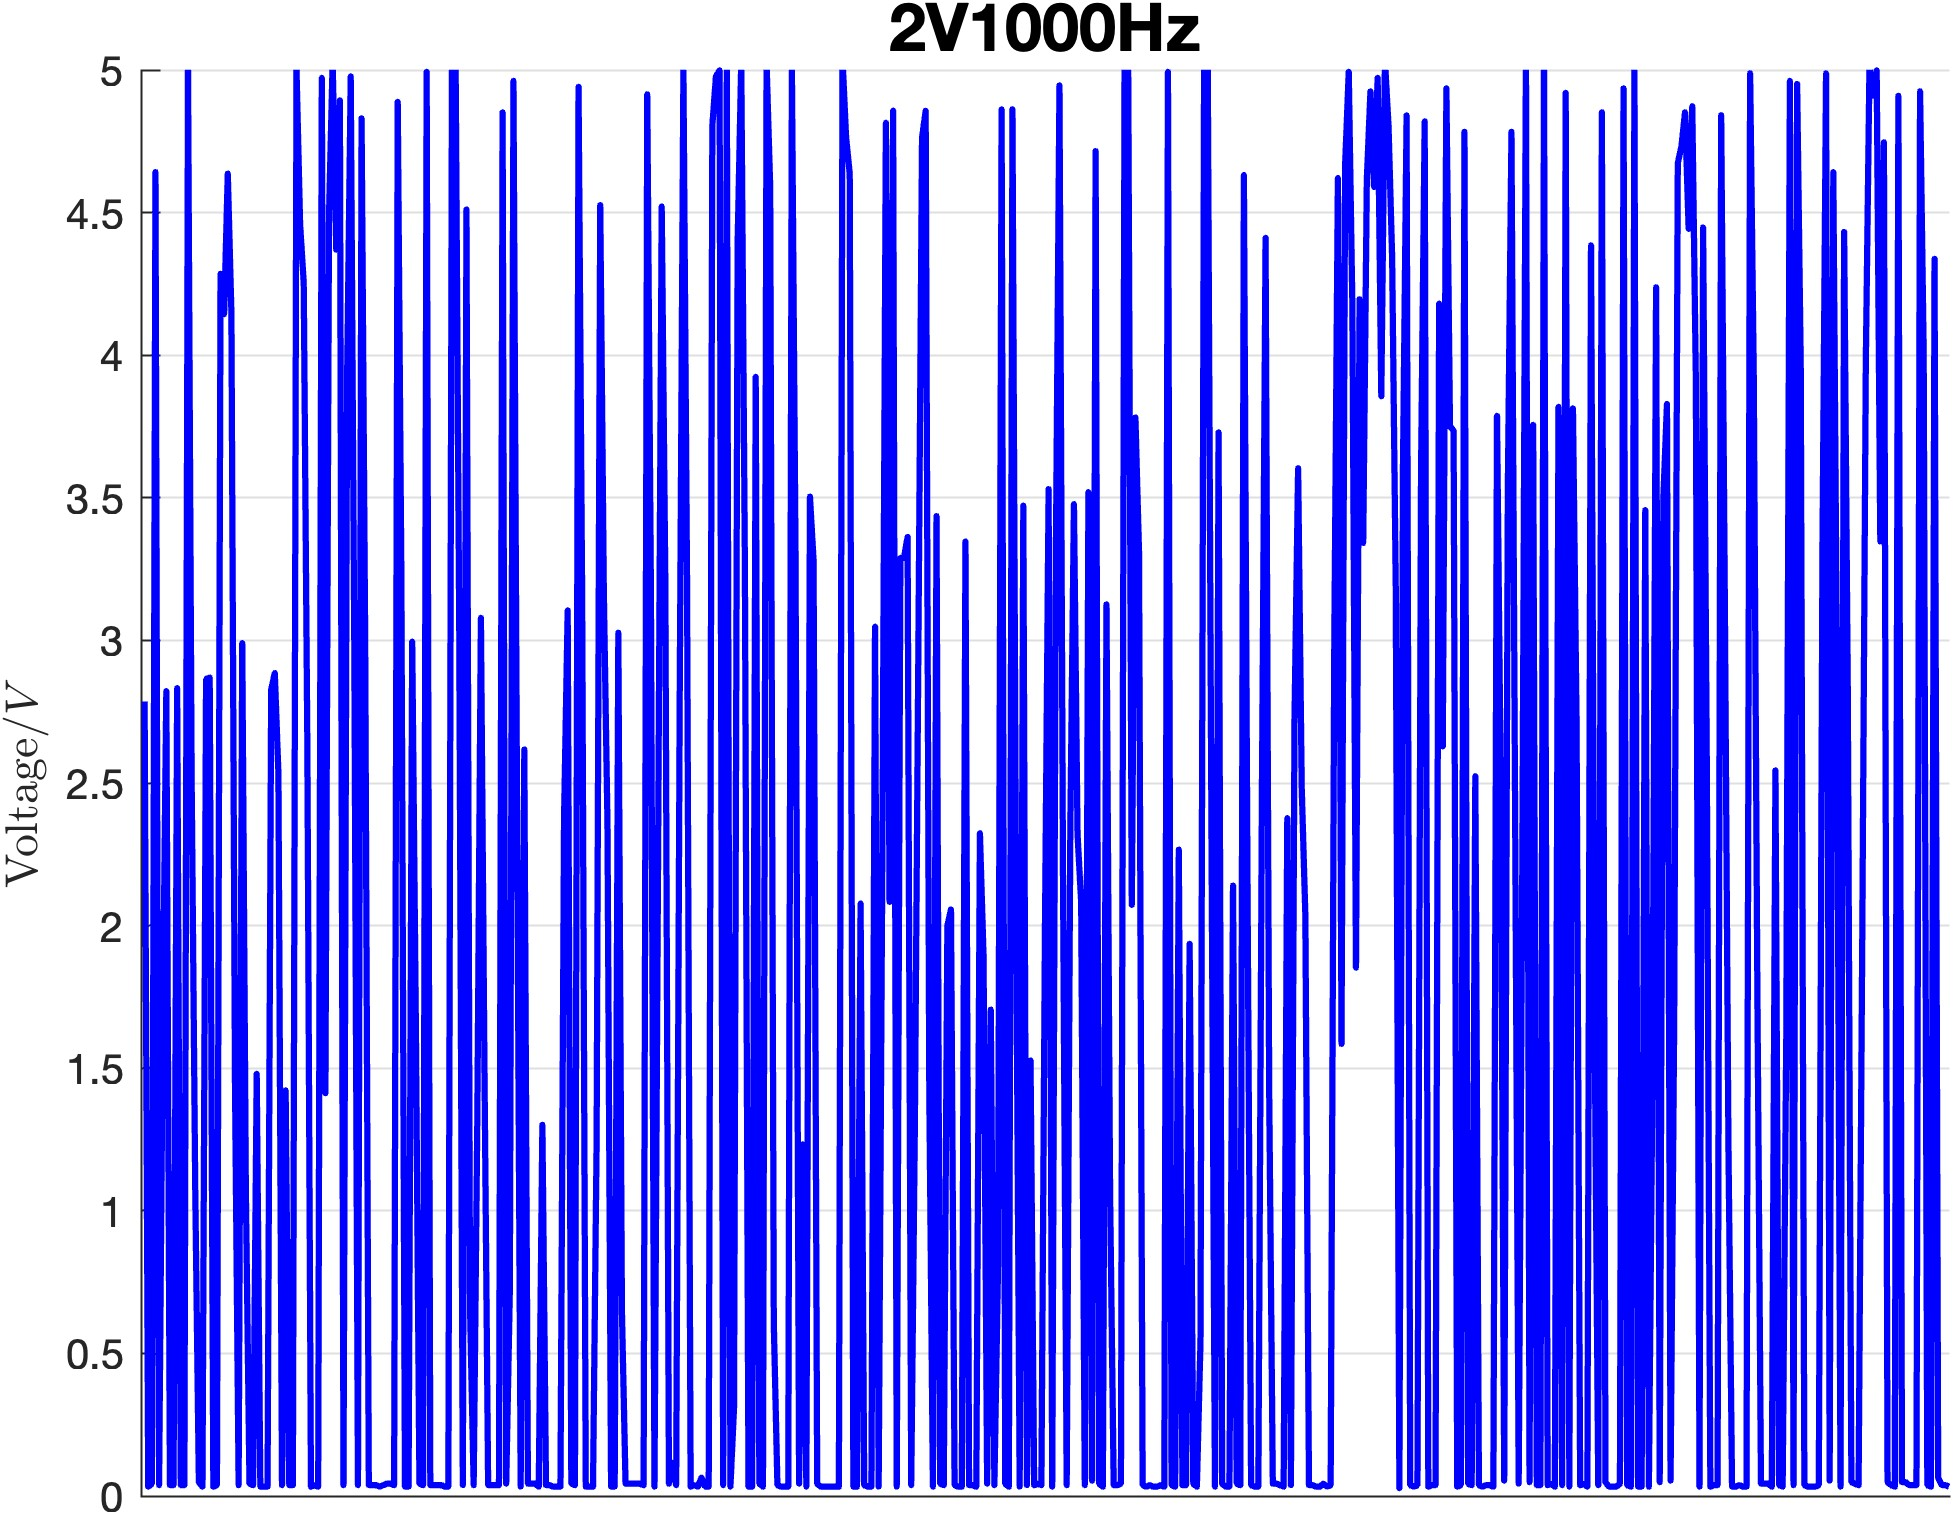
\includegraphics[width=\textwidth]{2V1000HzW.jpg}
            \end{minipage}
            \captionof{figure}{移除负反馈电容}
            \label{diffFreqW}
        \end{minipage}

        \item 分光光度计与碘钟实验
        \\[1mm]
        使用如图~\ref{Labview} 程序记录LED-PD电路输出电压，得到图~\ref{V-t}。
        \\[3mm]
        \begin{minipage}{\linewidth}
            \centering
            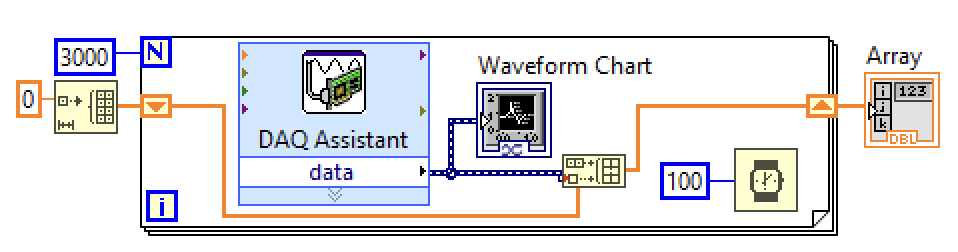
\includegraphics[width=0.85\linewidth]{Lab10.png}
            \captionof{figure}{Labview程序}
            \label{Labview}
        \end{minipage}
        \\[3mm]
        \begin{minipage}{\linewidth}
            \centering
            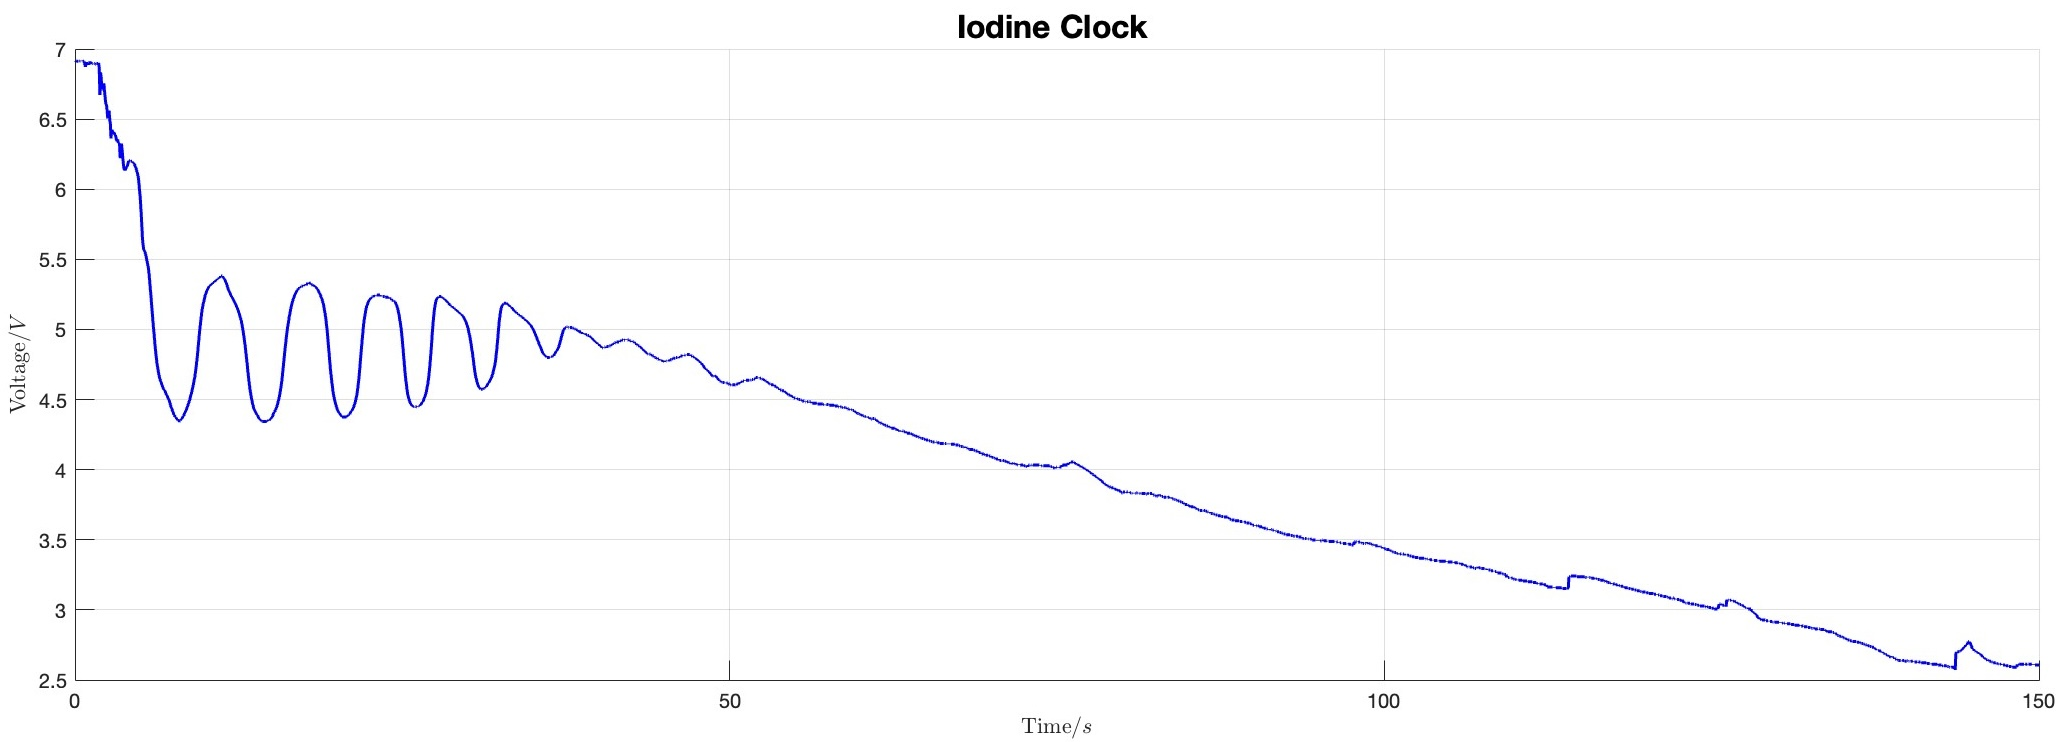
\includegraphics[width=0.85\linewidth]{Iodine Clock.jpg}
            \captionof{figure}{$V_\text{out}-t$图}
            \label{V-t}
        \end{minipage}
        分析曲线可知，反应大致可分为三个阶段。第一阶段为加入溶液A之前，此时比色皿中溶液为无色透明状态，透光度最高，电压稳定在$\qty{6.8}{\V}$左右；第二阶段为加入溶液A之后，反应进入震荡阶段，观察到反应共进行了五个完整的循环，每个循环周期约为$\qty{6.5}{\s}$；第三阶段为减弱阶段，此时丙二酸已基本消耗完全，碘单质不断生成并与淀粉结合，使得溶液颜色不断加深，透光度线性下降，输出电压也基本沿线性下降。下降过程中观察到曲线有小幅度震荡，可能是溶液中的气泡干扰了透光度变化。

        
    \end{enumerate}
\end{enumerate}
\end{document}